%%

%\documentclass[12pt]{article}



%\setlength{\textwidth}{16.5cm}

%\setlength{\textheight}{22.2cm}

%\setlength{\hoffset}{-.25in}

%\setlength{\voffset}{-.9in}


\documentclass[11pt]{article}
\usepackage{graphicx}
\usepackage{amssymb}
\usepackage{epstopdf}
%\usepackage{braket}
\usepackage[]{epsfig}
\DeclareGraphicsRule{.tif}{png}{.png}{`convert #1 `basename #1 .tif`.png}

\textwidth = 6.5 in
\textheight = 9.0 in
\oddsidemargin = 0.0 in
\evensidemargin = 0.0 in
\topmargin = 0.0 in
\headheight = 0.0 in
\headsep = 0.0 in
\parskip = 0.2in
\parindent = 0.0in

\clubpenalty=9999
\widowpenalty=9999

\setcounter{section}{1}



\begin{document}






\thispagestyle{empty}

\renewcommand{\thefootnote}{\fnsymbol{footnote}}




\begin{center}
\bfseries
\large{The Photon Beam and Detector for the GlueX Experiment}\\
\normalfont
\footnotesize{{\it GlueX Contribution - JLab Upgrade Technical Design Report}}\\
\small{\today}\\
\end{center}

\subsection{Overview}

The scientific goal of the GlueX project is to map the spectrum of gluonic
excitations starting with exotic hybrid mesons.  Photoproduction is expected to
be a  particularly rich venue for producing exotic hybrids which are predicted 
to have masses in the range from 1.5 to 2.5~GeV/$c^2$.  The optimal photon
energy is 9~GeV.  This energy is determined by the requirement that the mesons
be produced sufficiently above threshold so that resonance 
 line shapes are not distorted.  The $J^{PC}$ quantum numbers of exotic
 hybrids will be identified using an amplitude analysis that requires nearly
 $4\pi$ acceptance and sufficiently good resolution to identify exclusive
 reactions.  The need to establish decay modes also requires sensitivity to
 photons and charged particles whose species are identified.  The amplitude
 analysis also requires linearly polarized photons of sufficient flux (up to  $10^8$~photons/s)
  and this is
  achieved  using the  coherent bremsstrahlung technique.
 This sets the requirement that the electron energy be at least 12~GeV. 
 The discovery potential of GlueX depends on large statistics data sets what
 will be accumulated with a design rate capability of  100~MB/s.

\begin{figure}[h!]\centering
\begin{tabular}{c}
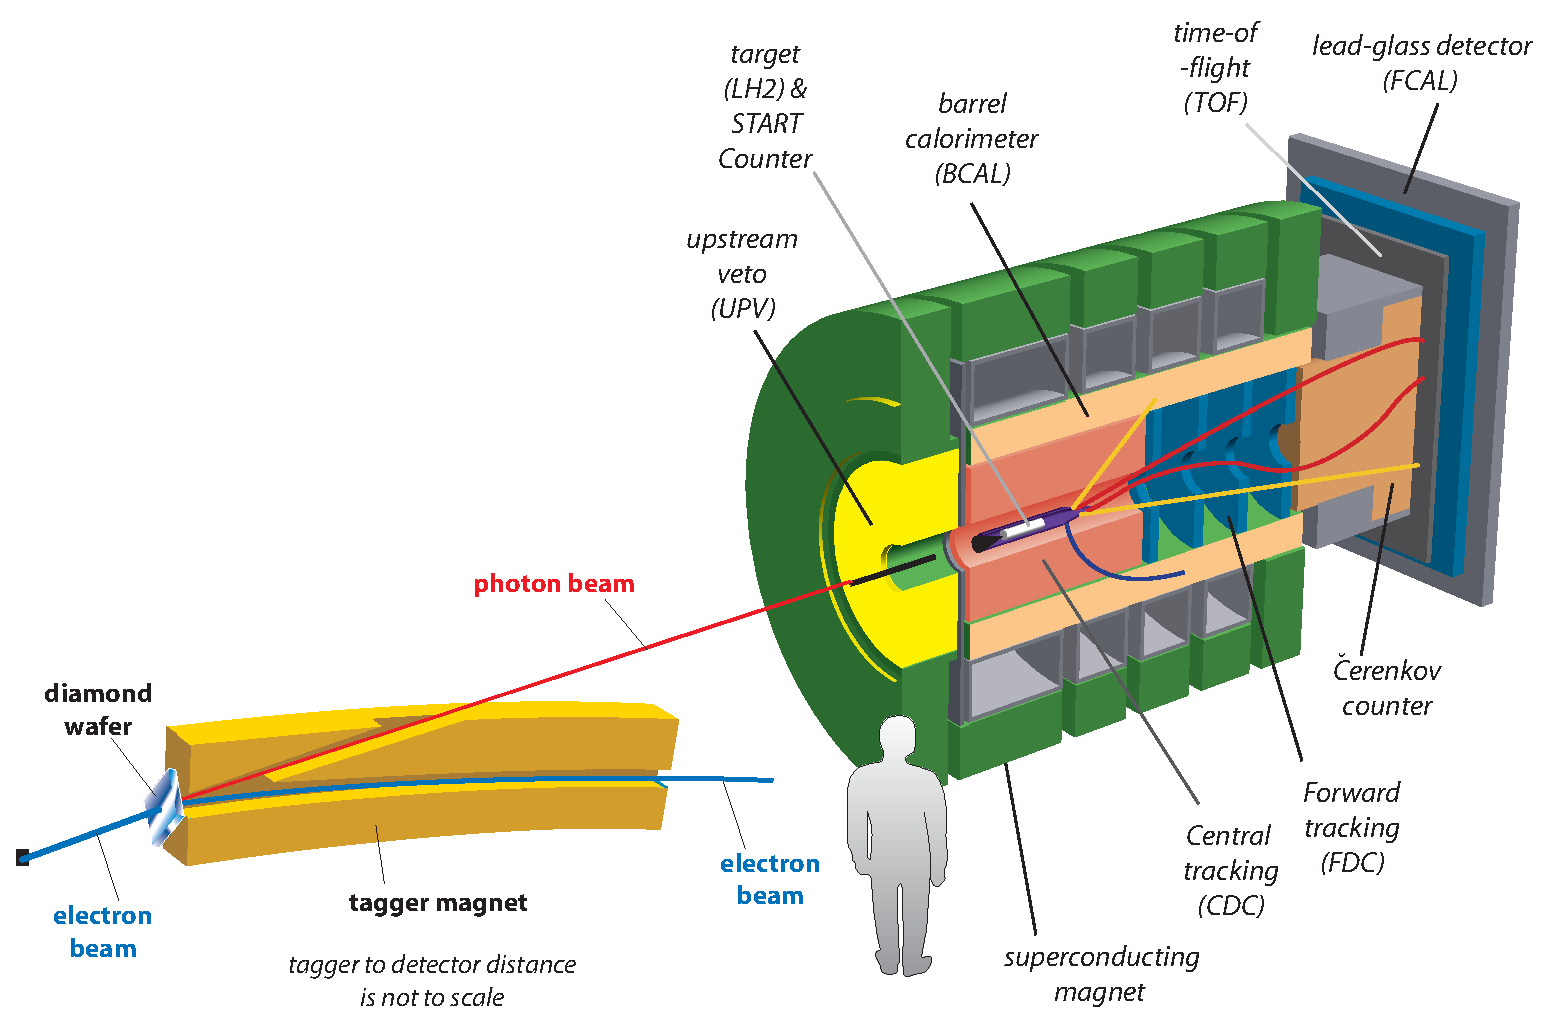
\epsfig{file= hd10.eps,width=0.95\textwidth}
\end{tabular}
\caption[Lecture 2]{\label{hd10}
Photon Beam Tagger and GlueX Detector.}
\end{figure}

\begin{table}
\caption[GlueX Detector Performance]
{\label{gluex_det}
GlueX Detector Parameters.}
\begin{center}
{\small 
\begin{tabular}{ll}
\hline
\hline
{\centering \textbf{\textbf{Parameter}}} & 
{\centering \textbf{\textbf{GlueX Performance}}} \\
\hline
\multicolumn{2}{c}{\emph{Charged Particle Detection}} \\
Coverage:             & $1^{\circ} < \theta < 170^{\circ}$\\
Momentum Resolution:  & $\sigma(p)/p=1-2\%$ \\
Position Resolution:  & $\sigma=150-200\ \mu$m \\
dE/dx measurements:   & $20\le \theta \le 140^{\circ}$ \\
BCAL time resolution: & $\sigma_t=250$~ps \\
TOF time resolution:  & $\sigma_t=60$~ps \\
$\pi/K$ separation: (Cerenkov) & $\theta < 14^{\circ}$ \\
\multicolumn{2}{c}{\emph{Photon Detection}} \\
Energy measurements:   & $2\le \theta \le 120^{\circ}$ \\
Veto:                 & $\theta \geq 120^{\circ}$ \\
BCAL resolution ($E_{\gamma}\geq$ 20 MeV):  & $\sigma(E)/E=(2+5/\sqrt{E})\%$ \\
LGD resolution ($E_{\gamma}\geq$ 100 MeV): & $\sigma(E)/E=(3.6+7.3/\sqrt{E})\%$ \\
BCAL  position resolution: & $\sigma_z=4$ cm \\
LGD  position resolution: & $\sigma_{x,y}=0.7$ cm  \\
\multicolumn{2}{c}{\emph{DAQ/Trigger}} \\
Level 1:     & 200 kHz at $10^{8}\gamma/s$\\
Event Rate: & 15 kHz to tape \\
Data Rate:   & 100 MB/s \\
\multicolumn{2}{c}{\emph{DAQ/Trigger}} \\
Fully pipe-lined &  FADCs and TDCs \\
\multicolumn{2}{c}{\emph{Photon Flux}} \\
Initially: $10^{7} \gamma/s$ & Final: up to $10^{8}\gamma/s$\\
\hline
%\hline
\end{tabular}
}
\end{center}
\end{table}

\newpage

Figure~\ref{hd10} shows a schematic of the GlueX detector.  The 12~GeV electron beam
is incident on a thin ($\approx$~20~$\mu$meter) thick diamond radiator.  The photon 
energy is determined by a tagging spectrometer with an energy resolution of 
0.1\%.  The detector is built around a superconducting solenoid that produces
central field of $\approx$~2~T.  The field is used to momentum analyze charged
particles and to contain within a cylinder of
small diameter  the electromagnetic background produced by the photon
beam interacting in the LH$_2$ target.  The target is surrounded by a 
START counter used in the level-one trigger.  Photons produced in the interactions
are detected and measured by the electromagnetic
calorimetry consisting of the upstream photon 
veto (UPV), the barrel calorimeter (BCAL) inside the magnet and a forward 
calorimeter (FCAL).  The UPV will mainly be used to veto backwards-going 
photons while BCAL and FCAL will be used to re-construct $\pi^0$ and
$\eta$ mesons.  Charged particle tracking consists of concentric cylindrical
layers of drift tubes in the central region (CDC) and planar drift chambers
in the forward region (FDC).  Particle identification will be realized using
time-of-flight using a forward wall of scintillators (TOF), timing information
from the  BCAL, additional particle identification from a threshold Cerenkov
counter and $dE/dx$ information from the CDC and FDC drift chambers.
These elements, along with the trigger, data acquisition (DAQ)
and software, are described in more detail below.
A more detailed drawing of the GlueX detector in side view is shown in 
Figure~\ref{gluex_det_3} and detector parameters are listed in 
Table~\ref{gluex_det}.

The GlueX detector design, along with its match to the physics requirements,  
was reviewed in 1999 and 2004.  The electronics was reviewed in 2003 and
the solenoid was reviewed in 2004. 
\footnote{Details of the design and capabilities of
the detector can be found at http://www.halld.org/cdr\_v5/index.html.}

\begin{figure}[h!]\centering
\begin{tabular}{c}
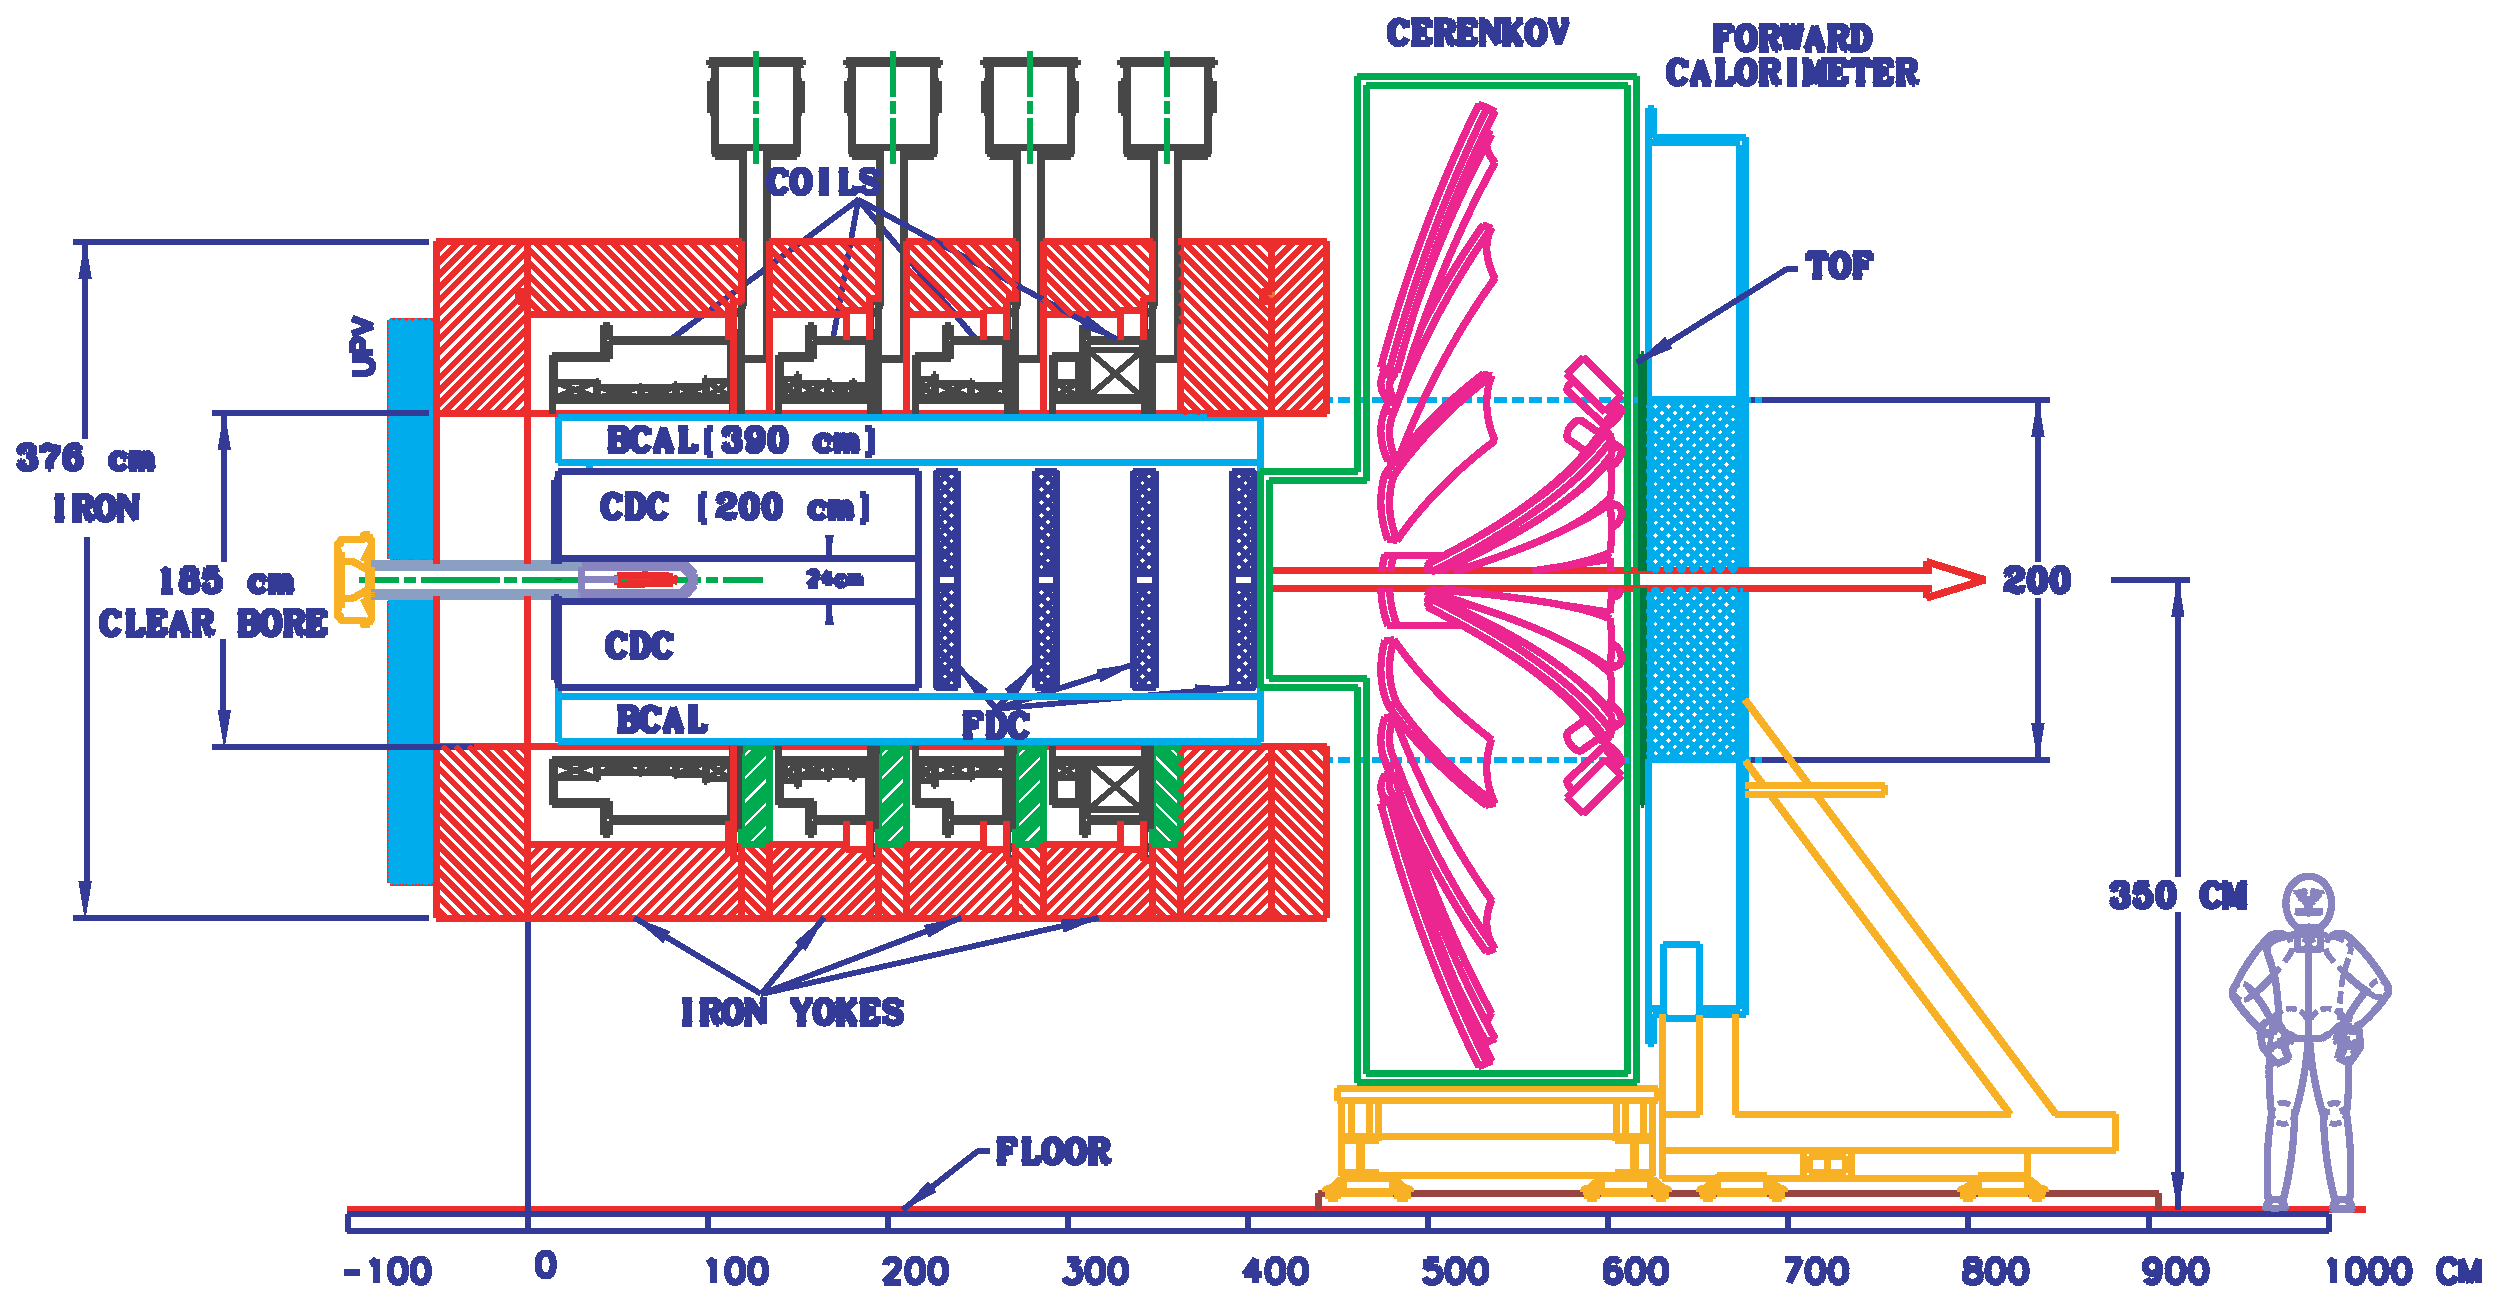
\epsfig{file= gluex_det_3.eps,width=0.95\textwidth}
\end{tabular}
\caption[Lecture 2]{\label{gluex_det_3}
GlueX Detector.}
\end{figure}


\subsection{Photon Tagger}

\paragraph{Purpose, Resolution Requirements, Description, Mass, Channel count}
The purpose of the Tagger system is to provide a flux of $\sim 10^{8}$~Hz
of linearly polarized photons from coherent bremsstrahlung in a thin,
orientated diamond crystal. This is achieved by measuring the energies
of the energy degraded bremsstrahlung electrons in the spectrometer.
The photon energy resolution is required to be less than 0.1\% r.m.s.\
of $E_{0}$ for $E_{\gamma}$ between 70\% and 75\%  of $E_{0}$, which
corresponds to 12~MeV r.m.s. energy resolution for a 12~GeV electron beam. 
The Tagger system consists of a quadrupole and 2 dipole magnets, 
a vacuum chamber and the associated focal plane detectors
as shown in Figure~\ref{ch4_taggerplan}. The dipoles
are two identical magnets that will be run at 1.5~T.  According to the
present design, the pole shoe surfaces will be part of the vacuum chamber.
The focal plane detector array is located just outside the vacuum chamber.
It consists of a set of 141 fixed scintillation counters spanning the full
energy range from 25\% to 95\% of $E_{0}$ and is required for the alignment
of the diamond. A movable \emph{microscope} of 120 narrow channels is required
to accurately measure the photon energies in the energy  range 70 to 75\%
of $E_{0}$.  The total mass of the tagging spectrometer system will be
$\sim$~90 tons.  

\begin{figure}[h!]\centering
\begin{tabular}{c}
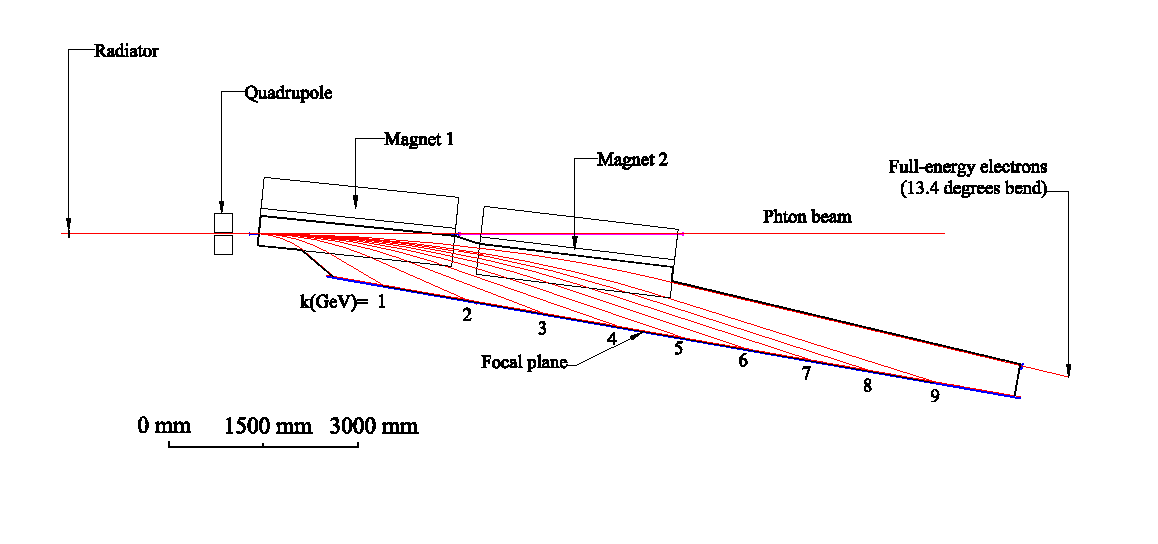
\epsfig{file= ch4_taggerplan.eps,width=0.85\textwidth}
\end{tabular}
\caption[Lecture 2]{\label{ch4_taggerplan}
A plan view of the tagging spectrometer from above, showing the
  path of the primary beam and the trajectory of post-bremsstrahlung
  electrons of various recoil momenta.}
\end{figure}

\paragraph{Raw Signals, Stages of Amplification, Final readout}

Since individual detectors in the focal plane array will have to count
at rates up to $5\times 10^{6}$~Hz, a plastic scintillator/photomultiplier
combination is appropriate.  The fixed scintillator array consists of
paddles 0.5~cm thick mounted perpendicular to the electron trajectories
which span 0.5\% $E_0$ each in recoil electron energy for a total of 141
counters.  The microscope consists of a rectangular array of square
scintillating fibers connected to clear plastic light guides.  Each
fiber is read out with a silicon photomultiplier device, which provides
excellent gain, rate capability and time resolution.  The signals from
the individual fibers are ganged together to form 120 independent tagger
channels of approximately 0.1~\% $E_0$ each.  The digitization electronics
from the focal plane detectors will be standard.


\paragraph*{R\&D Issues, Simulations and Other Considerations}
The Glasgow  and Catholic Universities groups have calculated the tagger
optics separately, the results of which can be found in Hall D
note 70\footnote{Optics calculation for the Hall D tagging spectrometer
for a 12 GeV electron beam. G. Yang, January 2004.} and the GlueX/Hall D
Design Report (Nov 2002). The Design Report tagger is different from
the design described above. It has a single long, narrow dipole which is
6.1 m in length and weighs $\sim$ 100 tons. Due to concerns about the
mechanical stiffness, the availability of sufficiently large pieces of
iron of the necessary quality and the availability of suitable
manufacturers, Glasgow  and JLab investigated the possibility of a
tagger consisting of two identical magnets in series\footnote{Optics
calculation for a two magnet tagged photon spectrometer for GlueX.
G. Yang, July 2004.}.
By  careful positioning of the two magnets it is possible to obtain a
design that is equivalent, and in some respects superior, to a single
magnet configuration. The two magnet design concept was accepted by
the collaboration at the Indiana meeting in May 2004. Glasgow has studied
the design in more detail and has produced drawings of the two magnet
assembly, including a possible vacuum system. This design has been submitted 
to a commercial manufacturer from whom a budget price has been obtained.
It is also relevant to mention that prior to version 4 of the Design Report, 
Glasgow and JLab investigated the feasibility of a tagger with superconducting 
coils\footnote{Possible designs for a 12 GeV superconducting Tagger. J. Kellie, 
November 2001.} with a magnetic field of 5T and main beam bend angles of 15, 30 
and 45 degrees, for both curved and straight output edges - the room temperature 
tagger bend is 13.4 degrees. After careful consideration, the superconducting 
option was rejected since there are several distinct disadvantages and no 
clear advantages. There will be a full review of the tagger and beamline, in October, 2005.

\paragraph*{Other Considerations}

The Tagger system has been the responsibility of groups from Glasgow 
University, JLab  and Catholic and Connecticut Universities.  More 
work is required to investigate alternative vacuum system designs,
of which several have already been considered. 


The Moscow group using ISTC financing could provide the necessary 
manufacturing skill and manpower to produce the magnets and the 
vacuum chamber.  A design engineer from IHEP is planning to visit 
JLab for 2 to 3 months in Autumn 2005 where he will participate in 
detailed discussions of the tagger with the JLab and Glasgow groups. 
Basic R\&D is required for the focal plane assembly. Catholic University 
will be responsible for the broad band focal plane and Connecticut 
University for the focal plane microscope, bearing in mind manpower requirements.

\subsection{Superconducting Solenoid}

\paragraph{Purpose and Requirements}

The Solenoid is the magnetic element selected for the GLueX Experiment to
provide momentum analysis in the tracking chambers. The Solenoid
is a 73-inch warm bore super conducting (SC) device that produces
a nominal maximum central field of 2.2~Tesla at 1800~Amps. The magnet is
195~inches long and weighs  approximately 300 tons. The solenoid was originally
 designed in 1970 as the Large Acceptance Solenoid Spectrometer
 (LASS) spectrometer at
SLAC and was subsequently used as the MEGA spectrometer at 
Los Alamos National Lab (LANL). The
solenoid was mothballed in place
in 1995 and first inspected by JLab/Hall~D in 2000. The solenoid was
designed as a highly reliable cryogenically stablized superconducting magnet.
The typical field quality of the solenoid (dB/B $\approx$ 1 \%) is consistent with GlueX
requirements for momentum resolution. The solenoid was
designed with a slotted yoke and four separate cryostats to accomodate 
the large planar wire chambers used at LASS.
The specific magnetic geometry of the original solenoid had the unfortunate 
side effect of
creating large external magnetic fields, particularly in regions where
phototubes would likely be present. Many of the solenoid's systems were
inconsistent with JLab operations due either to design or obsolescence.
The solenoid had a history
of internal leaks and electrical shorts and had accumulated a substantial 
amount of wear and tear during its 30 year history.
Despite these problems, the robust design and the good state of
preservation made the selection of this solenoid a cost effective
choice for Hall~D, even after the necessary costs of modernization and
maintenance were taken into consideration.

\paragraph{Status of Upgrading, Modernization and Repair}

 The first task
performed after the initial evaluation of the solenoid was to redesign the
yoke magnetic geometry to match the Solenoid to the requirements of Hall~D
and to reduce substantially the external fields. The proposed modifications
entail filling the yoke slots and adding steel at the end to reduce yoke
saturation and the escape of internal fields, thus reducing the external
fields by creating a symmetric yoke with a large upstream opening. This
modification also changed the solenoid to a clear bore from end to end.

The MEGA solenoid was dismantled and shipped to the
Indiana University Cyclotron Facility (IUCF) where it has been 
undergoing some long needed maintenance and repairs. Two of the four
coils are now finished. Refurbishment included repairing LN$_2$ leaks in three coils and a leak
in the LHe vessel of the forth. The shield thermometry is being upgraded to
modern PT-102 Pt resistance thermometers, and the coil support
strain gauges and the deteriorated multi layer super insulation are all being replaced.
The two completed coils were cooled down with
LN$_2$ in July 2004 to perform a final cold leak test and they were
determined to be leak-free to the highest industry standards. This cold testing also 
confirmed that the new instrumentation and insulation worked as designed. 

A mid-course assessment of the solenoid by external experts was held in December of 2004 to
provide advice and recomendations on the present course of restoration and future 
plans for the solenoid. The most significant recomendation was to consider actions 
to eliminate the coil shorts. This advice was taken to heart and a plan was 
concieved to perform a surgical short repair on coil~3 which has a  
hard short to ground. This extra work was incorporated into the work plan for coil 3,
and work on coils~3 and 4 is due to be completed in early 2006.

New solenoid systems are planned that include a new DC power
supply and energy dump system recently purchased from Danfysik for GlueX.
A new cryogenic interface with JLab compatible automatic valves and
connections and a new control and instrumentation package is under design at JLab.

\paragraph{Other Considerations}

The refurbishment of the coils is being performed at IUCF under
the direction of JLab staff, and will continue until complete.
A cost-benefit analysis is underway to determine the ultimate value 
of a full-scale test of the solenoid including the iron yoke 
in advance of the availability of Hall~D, possibly at IUCF.
Ultimately the solenod will be installed and thoroughly tested in Hall D 
prior to the installation of the actual GlueX apparatus. This installation
is one of the schedule drivers for the experiment, and therefore must be 
streamlined to allow prompt assembly of the detector.

\subsection{Target}

\paragraph{Purpose, Resolution Requirements, Description, Mass, Channel Count}
The main physics program for the GlueX experiment will be conducted with a
low-power liquid hydrogen target. The planned target is 30~cm long and
somewhere between 3 and 6~cm in diameter. Such targets normally 
employ mylar target cells. The mylar cell will be mounted on a metal base 
to provide for liquid entry ports and a reliable means of positioning the 
cell. The beam enters through a thin window mounted on a reentrant tube at 
the base of the cell. The target cell is connected to a condenser located 
upstream of the cell.

\paragraph{R\&D Issues, Simulations, Monitoring}
The maximum power deposited in the target by the beam is 100~mW.  In such low-power
targets, natural convection is sufficient to remove heat from the target cell and a
circulation pump is not required.

\paragraph{Other Considerations}

The target will be built by the JLab target group. It is estimated that
approximately one year will be required to design, construct, test and
certify the target. This target is very similar to other targets that
have been built at JLab, partcularly for Hall~B.

 A system such as this, containing a few hundred 
cm$^3$ of liquid hydrogen, would be considered \emph{small} by JLab standards
and the safety requirements would not place any significant constraints on the target
design or operation.



\subsection{Start Counter}




\paragraph{Purpose, Resolution Requirements, Description, Mass,
Channel Count} The start counter is used to provide a start signal for
time of flight measurements and to identify the beam pulse associated
with the observed event. In order to be independent of particle
momenta and trajectories, the start counter is located as close to the
target as possible. To be able to identify beam pulses the detector
needs a minimal time resolution of 300~ps. The detector is very useful in
the early stage of the experiment when the photon flux is of the order
of $10^{7} \gamma/s$.

The detector will consist of an array of about 6 scintillators
that surround the target,\ approximating a cylinder with a conical
downstream end. The cylindrical section is 55~cm long, with an inner
diameter of 11~cm and the conical section is 14.2~cm long while the
inner diameter is reduced from 11 cm down to 2~cm. Each scintillator
element will have a thickness of 2~mm. Monte-Carlo studies have shown
that multiple scattering in this detector limits the vertex resolution
along the beam to about 2~mm (FWHM) for particle trajectories with an
angle of ~7.5$^\circ$ with respect to the beam. For larger trajectory
angles the ultimate resolution falls below 1~mm. The rms multiple
scattering angle is increased by 2~mr for trajectory angles larger than
25$^\circ$. At this angle the target material alone contributes 2~mr.
For angles around 75$^\circ$ the target contribution increases to
5~mr while the detector still contributes only 2~mr.
A schematic drawing of the detector is shown in Figure~\ref{start}.

The detectors can be read out
either via high magnetic field PMT's or other detection methods based
on solid state detectors.


\begin{figure}[h!]\centering
\begin{tabular}{c}
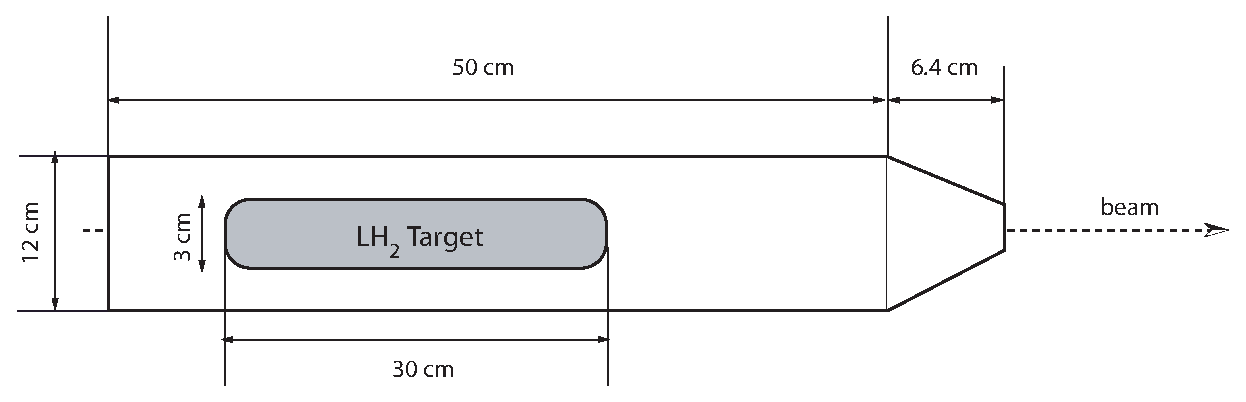
\epsfig{file= start.eps,width=0.5\textwidth}
\end{tabular}
\caption[Lecture 2]{\label{start}
GlueX START counter surrounding the LH$_2$ target.}
\end{figure}

\paragraph{Raw Signals, Stages of Amplification, Final Readout}
From studies using cosmic rays we have determined that high field
PMT's such as the Hamamatsu R5942 (H6614-01 system) can provide a time
resolution of 250~ps which makes is suitable for our application. For
minimum ionizing particles we obtained signal sizes of about 0.4~V
with a rise time of about 5-8~ns.

\paragraph{R\&D Issues, Simulations, Monitoring}
The timing performance of the Hamamatsu tube must be determined in
various magnetic field configurations. Other readout methods using
SiPM will also be studied.

\paragraph{Other Consideratio}
FIU is responsible for the start counter. In its current form, without
the need of high resolution position information, the available man
power at FIU is sufficient.
We expect that the counter can be built on the time scale of one year.

\subsection{Calorimeter -- BCAL}

\paragraph{Purpose, Resolution Requirements, Description, Mass, Channel count}
The purpose of the BCAL is the detection and energy determination
of photons and charged particles from the decays of the neutral
$\pi$, the $\eta$ and other mesons decaying into photons.  All
charged particles that fall within its volume as they are swept
by the magnetic field, mostly in the momentum range of 0.3 to 1.0~GeV/$c$,
will also be detected.  Spatial information can also be extracted
from the timing information relative to the two read-out ends of the 
BCAL and from the  information provided by the independent read-out cells in each end.
The design of the BCAL is based on that of the KLOE calorimeter at LNF
in Italy. The expected energy resolution for photons is
$\sigma(E)/E\approx 0.02+0.05/\sqrt{E}$, while the expected timing
resolution is $\sigma(t)\approx 200/\sqrt{E}$~ps.  BCAL parameters are
summarized in Table~\ref{bcalparams}.
The physical layout of the
BCAL is a ring consisting of $48$ modules (segments) at an inner radius
of 65~cm and an outer radius of 90~cm.   Thus, its  approximate thickness
is 25~cm corresponding to approximately $18-19$ radiation lengths. The nominal
length of each module is 400~cm.  Each module is constructed as a matrix
of $96$ double clad scintillating fiber optic strands (SciFi+IBk-s), embedded
on grooved Pb sheets of 0.5~mm thickness. Thus, each module consists of
approximately $220$ layers of Pb/SciFi and special optical epoxy composite.  The 
Pb:SciFi:Epoxy ratio (by volume) is 37:49:14.
The high magnetic field - and the limited space available for read out - present an 
area of particular concern and several emerging photo-detection technologies, such
as SiPM's, offer attractive solutions.  An intensive R\&D effort has been initiated in order
to finalize the type of readout devices and the required channels.

\begin{table}[h!]\centering
\caption{Main parameters of the Barrel Calorimeter.}
\begin{tabular}{|l|c|}
\hline
Parameter & Size \\ \hline
Length & 390 cm  \\
Inner radius & 65 cm  \\
Outer radius & 90 cm  \\
Fiber diameter & 1 mm  \\
Lead Sheet thickness & 0.5 mm \\
Number of Fibers & 1,000,000\\
Number of Readout Channels & $\sim$1000-5000 \\
Mass & 22 metric tons \\
\hline
\end{tabular}
\label{bcalparams}
\end{table}


\paragraph{Raw Signals, Stages of Amplification, Final readout}
It is clear that a large number of SciFi will be read out by any of the
selected PM's.  The exact number depends on the PM window size and its signal saturation
properties.   Assuming 1~mm$^{2}$ to 3~mm$^{2}$ SiPM window area and a 
5~cm~$\times$~ 5~cm matrix area viewed, approximately $1600$ SciFi's will 
be viewed by a number of SiPM's. The optimum number of SiPM's required will 
depend on the nature and geometry
of the light concentrator and diffuser and the light collection efficiency of
the optical fibers that will transport the light to the SiPM's.   Within a few months, the
first prototype sensor modules (matrices) of SiPM arrays mounted on a common
silicon wafer with integrated electronics will be available for testing.  These will need to 
be coupled to Winston cones as light guides.



\paragraph{R\&D Issues, Simulations, Monitoring}
The R\&D on the actual construction of the BCAL is almost complete with
a full-scale $4$~m module built, and tested with cosmic-rays.  The
read-out requires significant R\&D and MC simulations, more so because the SiPM
technology is still not yet mature and specifications and performance improve
with demand and experience.  This R\&D has already started and it is expected that
by the end of 2005 we will have the first test-beds of SiPM detectors with a large
effective viewing area to make them suitable for the BCAL.



\paragraph{Other Considerations}

The BCAL is the responsibility of the U of Regina SPARRO group.   For the construction
of Module 1 and subsequent production modules, as well as radiation damage
studies of the SciFi's, the CSR group at the University of Alberta is also
assisting.  This combined manpower is adequate to complete the R\&D phase
by the end of 2005.   It is also adequate to complete the construction of
the BCAL subject to external funding and adequate construction timelines.
The high-energy physics group at the University of Athens will be assisting
with the SiPM R\&D, as the European component of this emerging technology effort.

\subsection{Calorimeter -- FCAL}


\paragraph{Purpose, Resolution Requirements, Description, Mass, Channel Count}

The purpose of the FCAL is to detect and measure the energy and position of photons
from the decays of $\pi^0$, $\eta$ and other mesons.  LGD's of similar construction
were used in experiments at Brookhaven (E852 - using a pion beam) and JLab (Radphi
-using a photon beam).  
 The energy resolution
given by $\sigma(E)/E = 0.036 + 0.073/\sqrt{E}$.
Shower positions at the LGD plane
 are reconstructed with a resolution
 of $\sigma_r = \sqrt{(7.1/\sqrt{E})^2 + (X_0 \sin\theta)^2}$~mm
 where $X_0$ is the radiation length of the lead glass
 (30~mm) and $\theta$ is the photon angle measured with respect
 to the normal to the LGD (energies in GeV). This leads to mass resolutions of 10~MeV/$c^2$
 and 30~MeV/$c^2$ for the $\pi^0$ and $\eta$ respectively.
   The detector consists of 2300 lead
glass blocks of dimensions $4 \times 4 \times 45$~cm$^3$ arranged in a nearly circular
stack of radius $\approx$1~m.
  The Cerenkov light from each block is viewed by a FEU-84-3 Russian phototube. 
The phototube bases are of a Cockcroft-Walton (CW) design.  The phototubes are resigtered 
with respect to the glass using a cellular wall that includes soft-iron and $\mu$-metal
shielding. Since the LGD is the furthest downstream subsystem in the overall
GlueX detector, the mass presented to particles is not an issue.  The channel count is 2300.


\begin{figure}[h!]\centering
\begin{tabular}{c}
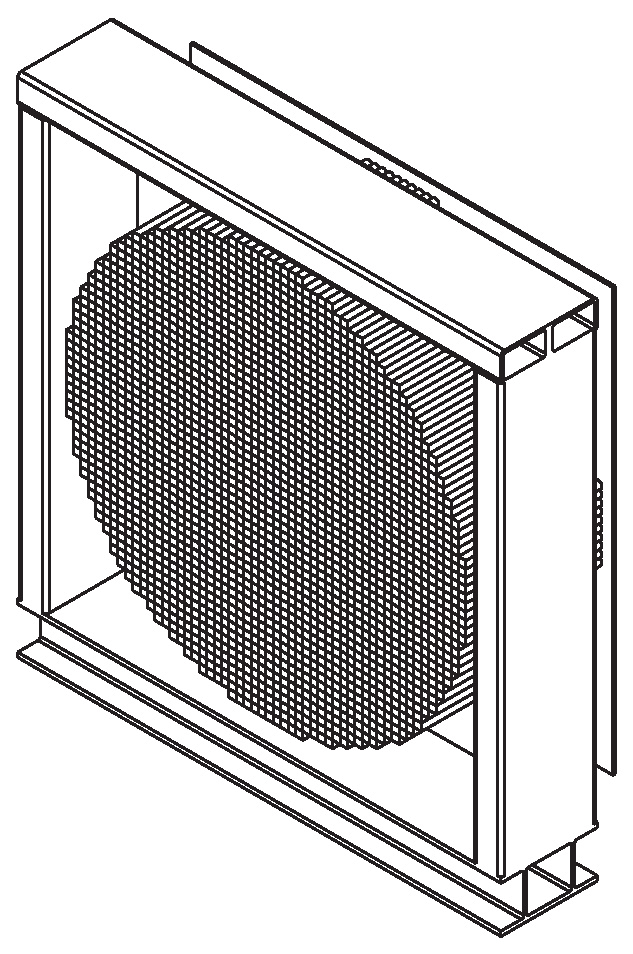
\epsfig{file= ch6_hd_pbglass.eps,width=0.4\textwidth}
\end{tabular}
\caption[Lecture 2]{\label{ch6_hd_pbglass}
The GlueX FCAL consisting of 2300 lead glass blocks.}
\end{figure}


\paragraph{Raw Signals, Stages of Amplification, Final Readout}

A 1~GeV photon produces about 800 photoelectrons corresponding to a phototube
signal of about 0.5~V and a rise-time of 10~ns.  No further amplification is required.  
The signal will be digitized with an 8-bit 250~MHz FADC.

\paragraph{R\&D Issues, Simulations, Monitoring}

The performance of the FCAL has been described in two NIM publications for E852 
experiment\footnote{Nucl. Instr. \& Meth. \textbf{A332} 419 (1993); 
 Nucl. Instr. \& Meth. \textbf{A387} 377 (1997)} 
and a a submitted NIM article for Radphi. An earlier version of the CW base is described
in another NIM
publication\footnote{Nucl. Instr. \& Meth. \textbf{A414} 466 (1998)}.  
GlueX R\&D has concentrated on
construction of 100 prototype improved CW bases, evaluation of  lead glass and FE-84-3
phototubes used in E852 and Radphi to determining suitability for use in GlueX.
Radiation damage was observed in the blocks used by Radphi but a heat treating
technique has been developed that returns the blocks to new condition.
98\% of the phototubes tested to date have proven satisfactory.
Simulations of detector response is based on extensive
experience with E852 and Radphi data analysis.  
Raphi experience is particularly important
as it involved operating an electromagnetic calorimeter in an bremsstrahlung
photon beam.
The monitoring system consists of a plastic scintillator sheet covering the 
up stream end of the glass stack and illuminated by fibers connected to a pulsed laser.  



\paragraph{Other Considerations}

The FCAL is the responsibility of the groups from Indiana University and the Institute for
High Energy Physics (IHEP) in Protvino, Russia.  This manpower is adequate to complete
remaining R\&D in six months and to complete the detector construction (including CW bases) in
two years from availability of funds.

\subsection{Calorimeter -- UPV}


\paragraph{Purpose, Resolution Requirements, Description, Mass, Channel count}

The purpose of the UPV is to detect backward going photons of energy greater than 20 MeV 
emerging from the target region (see Figure~\ref{ch6_upv-site}).
 The UPV provides the upstream coverage of the hermetic photon detection. The design of 
the UPV employs a traditional lead-scintillator sampling calorimetry.   The detector is 
able to detect multiple photons with fast detection and with timing information that may 
be utilized at the trigger level.

The UPV consists of 18 planes of scintillator alternating with first 12 layers of lead 
sheets (0.36 radiation length thick) then 6 layers of  lead sheets (0.72 radiation length thick). 
The expected energy resolution for incident photons is $\sigma(E)/E = 5\% + 8\%/\sqrt{E}$ at 
a $24\%$ sampling fraction. Each scintillator plane consists of 56 strips of 
dimensions 4.25 cm x 238 cm.  The effective area of each plane is approximately 
238 cm x 238 cm with a 25.5 cm central hole to allow for the passage of the beam. 
The total detector thickness is 8.91 radiation lengths.    


The scintillation light is collected and readout at both ends of a stack of 
lead-scintillator strips.  The dector consists of 56 stacks  resulting in 112 readout channels. 
Position resolution transverse to the strips will be achieved via moments analysis 
whereas longitudinal resolution will be achieved via left-right timing resolution.   




\begin{figure}[h!]\centering
\begin{tabular}{c}
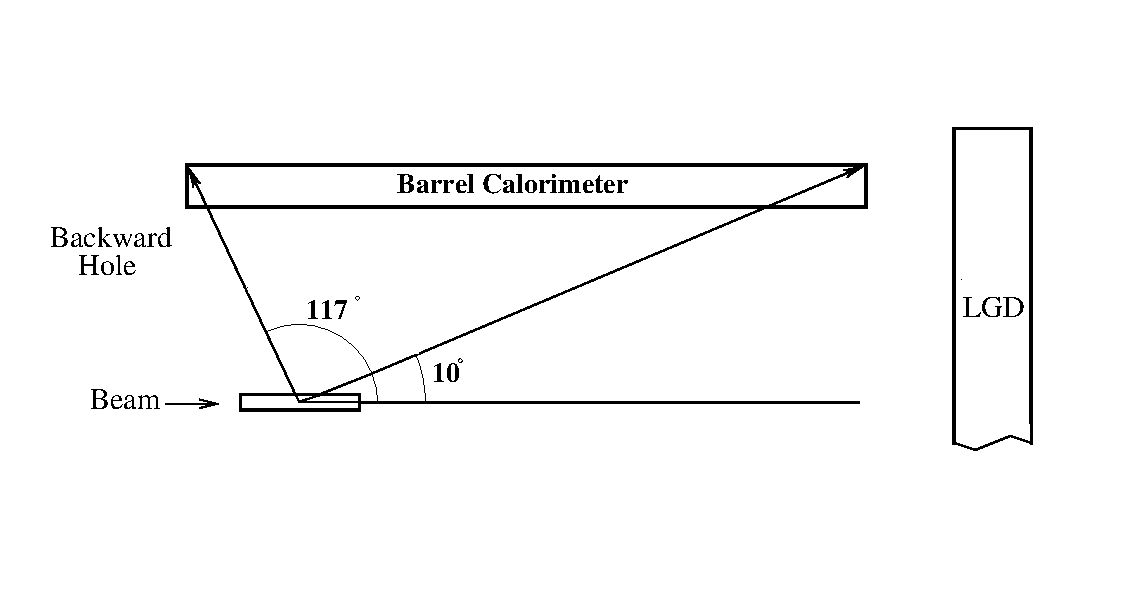
\epsfig{file= ch6_upv-site.eps,width=0.8\textwidth}
\end{tabular}
\caption[Lecture 2]{\label{ch6_upv-site}
Schematic showing the photon coverage of BCAL and FCAL.  The UPV is designed
to detect photons in the backward hole.}
\end{figure}

\paragraph{Raw Signals, Stages of Amplification, Final readout}

A typical pulse has a signal of 500 mV and a rise time of 10 nSec corresponding 
to about $10^3$ photoelectrons at $10^7$ PMT gain. The signal will be digitized 
using standard FADC and TDC modules.  

\paragraph{R\&D Issues, Simulations, Monitoring}

Initial R\&D on the construction and building techniques of a prototype module is 
near completion. Measurements of prototype performance in a low energy electron 
beam are planned for later this year.  These results will be compared to Geant4 
simulations.   R\&D continues on optimizing light collection, channel segmentation, 
and read-out. SiPM's, an emerging technology which is being studied for use in the BCAL, 
offer an attractive read-out solutions along with potential benefits in light collection 
and in minimizing high magnetic field effects. The monitoring system of the UPV read-out 
can be tied into the system utilized for the BCAL detector. A pulsed laser-fiber optic 
system is planned BCAL read-out devices.



\paragraph{Other Considerations}

The UPV is the responsibility of the group from Florida State University.  This manpower is 
adequate to complete remaining R\&D and to complete the detector construction 
in two years from availability of funds.

\subsection{Particle Tracking -- CDC}

\paragraph{Purpose, Resolution Requirements, Description, Mass, Channel count}

The purpose of the CDC is to accurately measure $(r,\phi,z)$
coordinates along charged-particle tracks. In conjunction with the FDC, it
will then  reconstruct the momentum, $\vec{p}$ of each track and the primary and
secondary vertices's of the event. The exact momentum resolution is a function 
of particle momentum and the number of hits in both the CDC and FDC. Monte Carlo
studies indicate that an $r\phi$-spatial resolution, $\sigma_{r\phi}$, on the 
order of 150 to 200~$\mu$m is sufficient to satisfy the physics goals of the 
experiment. The $z$-coordinate is obtained using $6^{\circ}$ stereo layers. 
The resolution is given as $\sigma_{z}=\sigma_{r\phi}/\sin 6^{\circ}$.  
The CDC also needs to provide dE/dx information sufficient for separating 
$K$s and $\pi$'s for particle momentum under 0.5~GeV/$c$.



\begin{figure}[h!]\centering
\begin{tabular}{c}
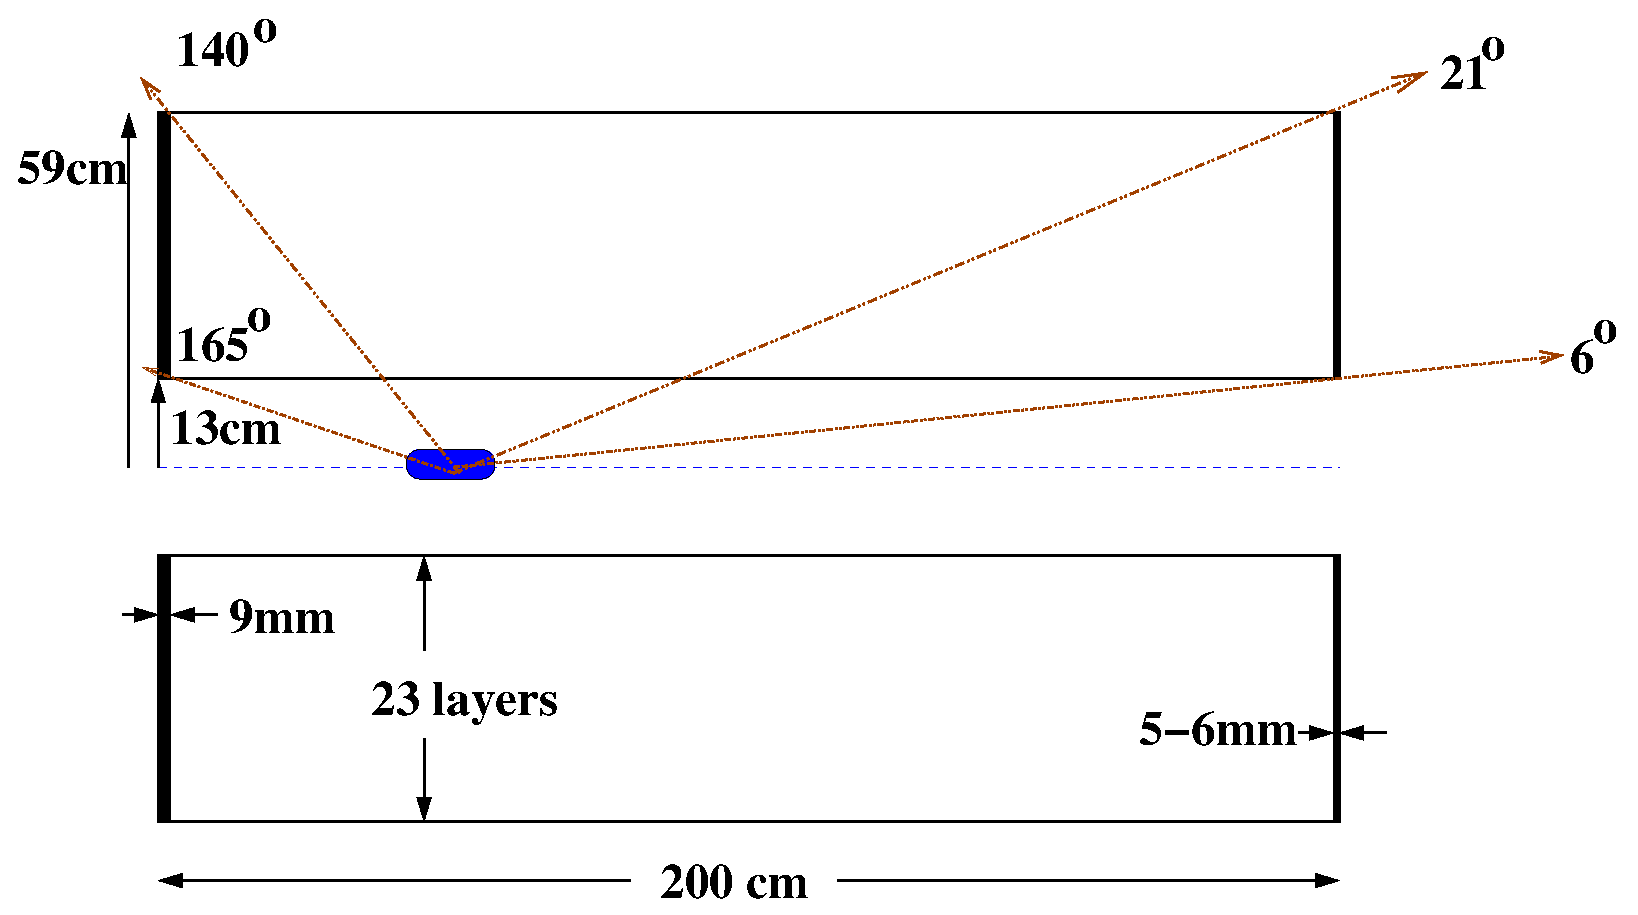
\epsfig{file= ch6_cdc_new.eps,width=0.8\textwidth}
\end{tabular}
\caption[Lecture 2]{\label{ch6_cdc_new}
A side-view sketch of the CDC.}
\end{figure}

The chamber is built using 23 layers of 1.6~cm diameter, 100~$\mu$m-thick
aluminized kapton, 2~m-long straw tubes. The signal is measured using a
$20\mu$ diameter gold-plated tungsten wire strung under 55~g of tension.
Layers $5$, $6$, $14$ and $15$ are $+6^{\circ}$ stereo while layers
$7$, $8$, $16$ and $17$ are $-6^{\circ}$ stereo. Due to the packing of the
tubes, the exact channel count depends on the exact specifications of the
final chamber, but is presently estimated to be $3240$ channels.

\paragraph{Raw Signals, Stages of Amplification, Final readout}

A minimum ionizing track produces about $30$ primary ionizations per 
centimeter of traversed gas. Path length in a straw-tube depends on
both the distance away from the wire as well as the polar-angle $\theta$
of the track, but typical values vary between about 0.5~cm to a few cm.
The chamber will be run such that the gas amplification is about $10^{4}$.
The signals will be read out using capacitively coupled preamps mounted
directly on the upstream end plate of the detector and then fed into 10+ bit
FADC and digitized at 125~MHz. Due to the 2.25~T magnetic field, the maximum
drift times will be on the order of 800~ns for a typical gas mixture. 


\paragraph{R\&D Issues, Simulations, Monitoring}

The group is currently stringing wires in a $\frac{1}{4}$-chamber, full-scale 
prototype. We have currently identified several design changes that will
facilitate easier construction. Apart from construction technique, the main
 issues to be resolved with the prototype are gas distribution and electronic
hook-ups.  


\paragraph{Other Considerations}

The CDC is the responsibility of the Carnegie Mellon University group. Assuming that
a team of stringers is hired during the actual fabrication phase (as has been
done with other chamber projects), the group has sufficient manpower to build the
final device on a time scale of three and a half years from the time that funds
become available. The group expects to work with the FDC team and the JLab electronics
group to build a preamp that is common to all chambers in the experiment.  


\subsection{Particle Tracking -- FDC}

\paragraph{Purpose, Resolution Requirements, Description, Mass, Channel Count}

The FDCs include 4 separate packages of disk-shaped horizontal drift chambers 
to measure the momenta of all charged particles emerging from the target at 
angles of up to 30$^{\circ}$ relative to the photon beam line.  Each package
consists of 6 planes of alternating anode and field-shaping wires with a 
wire-to-wire separation of 5~mm (119 anode wires per plane) and with 150~$\mu$m 
spatial resolution from the drift time readout.  Each wire plane is sandwiched 
between 2 planes of cathode strips (238 strips per plane with 5~mm pitch).  By 
charge interpolation of the electron avalanche image charge in the cathode strip 
readout, spatial resolutions at the cathode planes are expected of better than 
150~$\mu$m.  The strips are arranged in a $U$ and $V$ geometry with respect to 
the wires (at $\pm$45$^{\circ}$) allowing for separation and assignment of 
multiple hits within a chamber to the different tracks.  Adjacent chamber 
elements will be rotated by 60$^{\circ}$ with respect to each other in order 
to improve track reconstruction decisions on the corresponding anode wire 
left/right ambiguities, hence improving the overall resolution.  The wires 
that cross through the beam line will be deadened out to a radius of 3.5~cm 
to reduce the rates.  Each FDC package has a channel count of 3570, leading 
to a total channel count for the full FDC system of 14280 (2856 anodes and
11424 cathodes).

\paragraph{Raw Signals, Stages of Amplification, Final Readout}

Each signal from the FDCs (anodes and cathodes) will be sent to a
chamber-mounted charge-sensitive preamplifier that drives a pulse-shaping 
amplifier. The signals from the anode wires that are above some 
pre-determined voltage threshold will be discriminated and then digitized 
by 125~ps LSB resolution F1 TDCs.  The signals from the cathodes will be digitized with 
62.5~MHz 10-bit flash ADCs.

\paragraph{R\&D Issues, Simulations, Monitoring}

The primary development issues that must be addressed for the FDC system
are factors affecting the intrinsic resolution of the chambers, along with 
the mechanical and electronics layout.  The goal is to construct a tracking 
detector that meets the required design specifications and has a long life 
time, a uniform and predictable response, a high efficiency, and is 
serviceable in case of component failure.

Two detector prototypes will be completed and studied over the course
of the next three years.  The first will be employed to study the optimal 
electrode configuration for the system.  A second full-scale prototype
will be completed to test mechanical support designs for the chamber 
cathode planes and wire planes, which is necessary to avoid electrostatic 
instabilities and non-uniformities that are known to affect resolution. 
This second prototype will also be essential to complete the final design 
of the FDC circuit boards.  A significant aspect of the design work includes 
development and study of Monte Carlo of the GlueX detector system focussing 
on the properties of the FDC system that will enable us to meet or exceed 
the required design specifications.

The detector group at Jefferson Laboratory is developing the gas system
for the entire GlueX experiment.  The Ohio University group will work
to ensure that this design is adequate for the control and monitoring
of the FDC system.

\paragraph{Other Considerations}

The  FDC prototyping and design is primarily the responsibility of
the Ohio University group, with important support from the detector
group at Jefferson Laboratory.  The manpower available is adequate
to complete the detector R\&D within 3 years and to complete the
detector construction with 4 years pending availability of funds.



\subsection{Particle Identification -- Cerenkov Counter}



\paragraph{Purpose, Resolution Requirements, Description, Mass, Channel count}

The Cerenkov detector is to serve as part of the particle identification system
together with the time-of-flight system for forward-going charged particles.
The goal is to distinguish between pions, kaons and protons with
momenta above the reach of the time-of-flight system. Here we describe the gas
Cherenkov detector, one of two options considered for this task.
 
The gas Cerenkov counter operates as a threshold detector, tagging relativistic
pions above the threshold for emission of Cerenkov light. Several radiator materials have
been considered for the design. A pressurized gas radiator has the flexibility of
matching the index of refraction to the desired momentum range, but requires
thick gas containers in the downstream detector region. Two atmospheric-pressure
radiators were found to produce high acceptance rates: aerogel (n=1.008) and C$_4$F$_{10}$
(n=1.0015). The C$_4$F$_{10}$ radiator was selected because it has a momentum
threshold for pions of 2.5~GeV/$c$.

The proposed optics collects light from two sets of mirrors, which focus
the light onto 40 photomultiplier tubes. All forward particles detected by the
time-of-flight system and lead glass detectors will traverse one set of 
mirrors. Therefore, there is a hight premium for producing these mirrors with
minimal thickness.  A schematic of the
GlueX \v{C}erenkov   is shown in Figure~\ref{ch6_cherenkov}.




\begin{figure}[h!]\centering
\begin{tabular}{c}
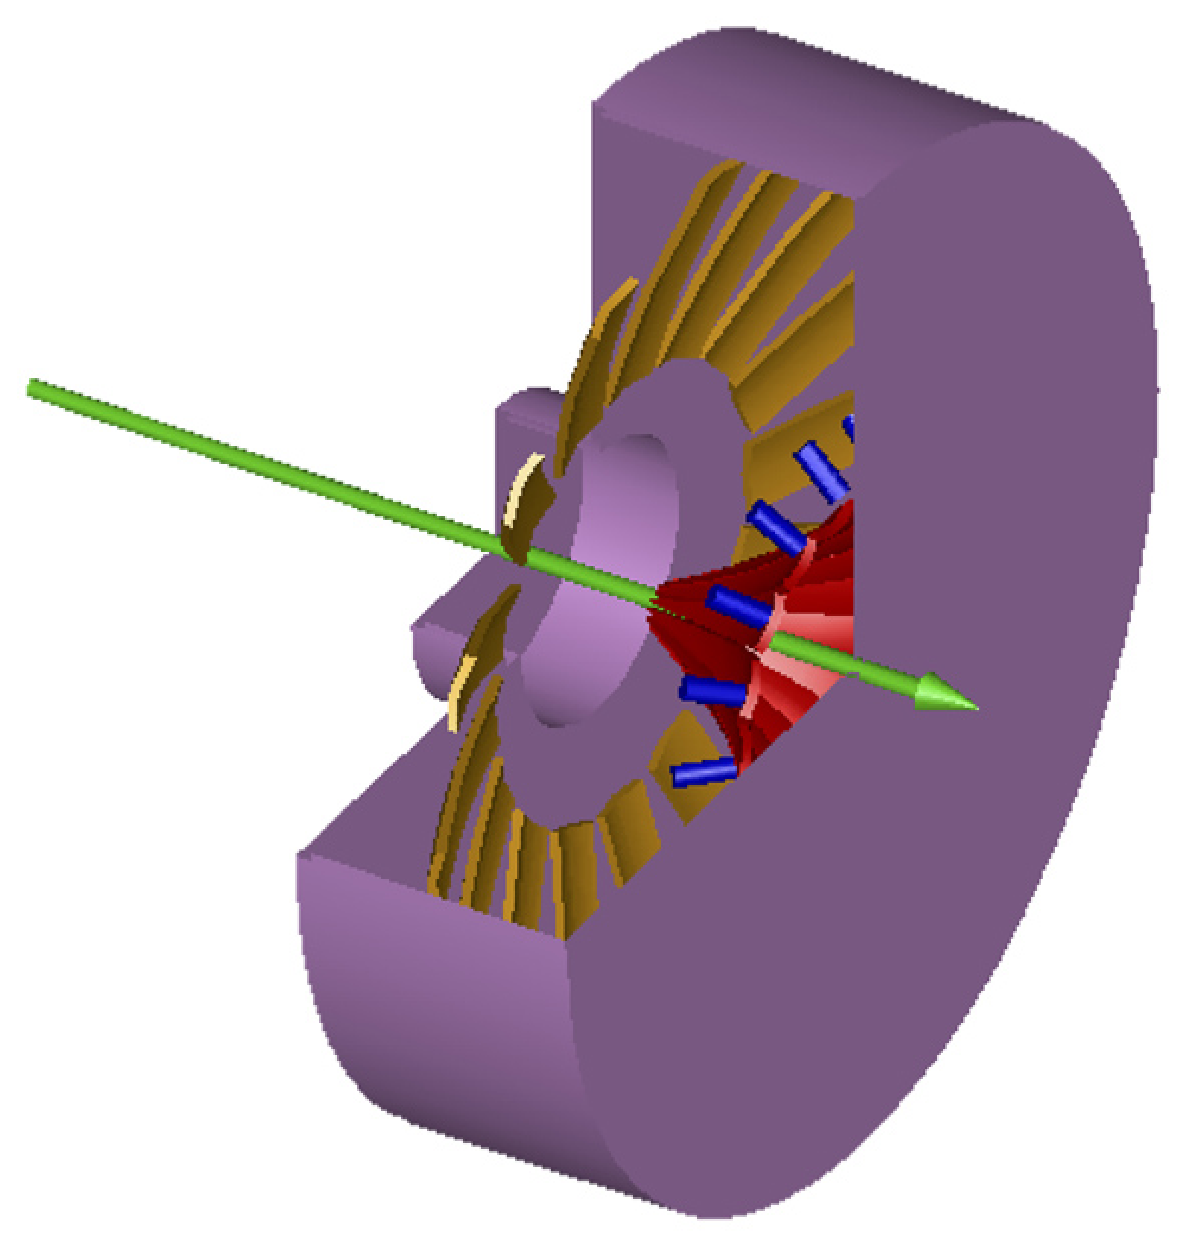
\epsfig{file= ch6_cherenkov.eps,width=0.5\textwidth}
\end{tabular}
\caption[Lecture 2]{\label{ch6_cherenkov}
A schematic drawing of the GlueX \v{C}erenkov detector system. The 
particles enter from the left into the gas volume in the center. The
\v{C}erenkov light is then reflected off the mirrors in the center 
(shown in dark) into the phototubes at the outer rim (shown as 
dark cylinders).}
\end{figure}




\paragraph{Raw Signals, Stages of Amplification, Final readout}

The performance of the system is expressed in terms of the average number
of photoelectrons detected per track. The radiator thickness is a minimum
of 80 cm of gas. A reasonably good design will produce
approximately 22 photoelectrons in the relativistic limit. For 95\%
detection efficiency, this sets the effective threshold of pions at  3~GeV/$c$.
The photomultiplier tubes will be placed about one meter away from the
opening of the solenoid, so special care will be required to
shield the photomultiplier tubes from the the fringe fields of the magnet.

\paragraph{R\&D Issues, Simulations, Monitoring}

Gas-filled Cerenkov detectors have been used in many particle physics 
experiments. Still, it is a challenge to collect
sufficient light for efficient detection of relativistic
particles. Many requirements must be balanced to achieve high efficiency.
The optics must to be designed to collect light to locations
where photomultiplier tubes can be placed and operated in the fringe
fields of the magnet. At the same time, the mirrors must have high reflectivity for the UV Cerenkov
photons as well as be thin to have minimal impact on particle trajectories.
The choice of radiator is also another variable. For example, the 
original LASS spectrometer used a freon radiator in a 
similar design to GlueX, but there is a limited selection of heavy
environmentally friendly gases. 

\paragraph{Other Considerations}

The Cerenkov detector for GlueX is not as well developed as other detector components.
This is due to the fact that the first group to express interest in this detector
is no longer part of the collaboration. However, after the granting of CD0 to the JLab 
upgrade, a pair of groups from Tennessee approached the collaboration and are eager to 
take on the responsibility for a major detector. Based on a fresh look at the challenges
for particle identification and their own expertise, they have proposed the
construction of a DIRC detector which is a very good match to particle identification
in this momentum range. A final decision on the detector technology we will use clearly
depends on many factors including physics, manpower, costs and timescales. The collaboration
is currently evaluating all of these.




\subsection{Particle Identification --TOF}

\paragraph{Purpose, Resolution Requirements, Description, Mass, Channel Count}

The purpose of the TOF is to serve as part of the particle identification system in conjunction with a Cerenkov
detector for forward-going charged particles.  The goal is to separate $\pi^{\pm}$ from $K^{\pm}$ for momenta up to
2~GeV/$c$ and  for the given geometry a 95\% separation efficiency is achieved  at the highest momentum with a time
resolution of 80~ps.  The TOF will use two planes of scintillator bars located immediately upstream of the lead
glass detector (LGD).  Based on simulations and prototype studies the bars will be 250~cm long, 6~cm wide and
1.27~cm thick.  Thus the mass presented by the  detector immediately before the LGD corresponds to 2.54~cm of
scintillating plastic. Each bar is read out at both ends with a photomultiplier.  The channel count is 168.

\paragraph{Raw Signals, Stages of Amplification, Final Readout}

Prototype studies with a cosmic ray test facility at Indiana U and extensive tests in a hadron beam at IHEP
(Protvino, Russia) included various scintillating bars of different thickness (1.25~cm, 2.5~cm and 5.0~cm) with
various photomultipliers (Russian FEU-115, Hamamatsu R5506 and R5946, and Philips XP2020).  The XP2020 was
chosen.   The typical pulse has a rise-time of less than 5~ns and an amplitude of about 0.5~V.  Constant fraction
discriminators will be used and  a TDC with a least count of 50~ps.

\paragraph{R\&D Issues, Simulations, Monitoring}

The performance of the prototype TOF in a 5~GeV/$c$ hadron beam at IHEP has been described in three NIM 
publications\footnote{Nucl. Instr. \& Meth. \textbf{A478} 440 (2002);  Nucl. Instr. \& Meth. \textbf{A494} 495
(2002); Nucl. Instr. \& Meth. \textbf{A525} 183 (2004) }.  For the 1.25~cm thick TOF bar, a time resolution for a
two-bar system of 77~ps at the bar center and 40~ps near the ends was achieved.  Magnetic shielding studies were
also carried out and are described in a NIM publication\footnote{Studies of magnetic shielding for phototubes;
accepted and available online at www.sciencedirect.com 10 Aug 2004}.  Further R\&D measurements with an array of
scintillator bars are planned for a pion test beam at TRIUMF in June 2005 and again in a higher energy hadron beam
at IHEP in December 2005.


\paragraph{Other Considerations}

The TOF is the responsibility of the groups from Indiana University and the Institute for High Energy Physics
(IHEP) in Protvino, Russia.  This manpower is adequate to complete remaining R\&D in six months and to complete the
detector construction in one year from availability of funds.


\subsection{Electronics}

\paragraph{Purpose, Description}

The electronics will amplify, discriminate, and digitize raw detector signals
storing them for later readout at level 1 trigger rates of 200 kHz
without incurring deadtime.  The detector includes
approximately 18,600 ADC channels and 6,300 TDC channels.

A pipelined approach is required due to the high trigger rate.  The
digitized information must be stored for several $ \mu s $ while the
level 1 trigger is formed.  Multiple events must be buffered within
the digitizer modules and read or transmitted while the front ends continue to
acquire new events.  The raw data rate from the detector is about 1
Gbyte/second. A sophisticated timing system is required to synchronize the
pipelines in the front-end modules.  The plan is to clock all digitizers in synchronization
with the accelerator timing.

Energy sums from the calorimeters as well as track counts from the barrel and TOF systems
compromise the level 1 trigger.



\paragraph{Current Status, R\&D issues}


Since no currently available commercial solutions exist the 
preamps, discriminators, digitizer modules, and timing system
will be designed by GlueX.

JLab has designed a multi-channel TDC module based on the ACAM TDC-F1
chip, and 100 units are currently in use in existing JLab experiments.  A high density
FADC with auxiliary user-definable processing is currently being developed at
Jefferson Lab.

A single-channel prototype 8-bit 250~MHz FADC, suitable for the barrel
and lead glass calorimeters, has been constructed at Indiana
University.  A multi-channel version which includes the energy sum is
currently being designed.

 A prototype constant-fraction discriminator has been built at the University of Alberta.

Preliminary work has been done on the preamps and
the timing system, and on a slower FADC for the tracking chambers.




\paragraph{Review}

The GlueX electronics system was reviewed in July of 2003.  The
reviewers concluded the basic design is sound and appropriate assuming
adequate human and fiscal resources.

The reviewers recommended that the work on the TDC and FADC should
continue.  A multi-channel FADC needs to be prototyped and evaluated.
As part of the level-1 trigger, the digitized calorimeter signals are
summed in a pipelined adder tree; the prototype FADC needs to
demonstrate this capability.

Analog front-end requirements need to be settled.  Prototype work
needs to begin, especially on the tracking chamber electronics to be
located inside the magnet.  The pipelined level-1 trigger, timing,
synchronization, and calibration systems all need further development.



\paragraph{Collaboration Responsibilities}

Indiana University and JLab have the major responsibilities for the
FADCs and TDCs, respectively. Still, 
the reviewers concluded that current manpower resources are
inadequate.  The University of Alberta has recently joined the
collaboration, but additional institutions possessing electronics
expertise are needed.  Discussions are under way with the Indiana University
Cyclotron Facility.

The reviewers also noted that a rudimentary management plan exists, but
that it needs further development.  
They estimated that the GlueX electronics effort could
require 6 years to complete after CD-3; the collaboration hopes to
reduce this time.  One possibility is a commercial partner/collaborator.



%======================== DAQ System =========================

\subsection{DAQ System}



\paragraph{Purpose, Description}



The GlueX experiment requires an LHC-era state of the art data
acquisition system, and the architecture is being designed for a flux
of $10^8$ photons/sec, Although at experiment startup the incident
flux will only be $10^7$ photons/sec, the architecture must be
appropriate for the full flux to avoid a costly redesign.  The
architecture scales such that components can be added as needed as the
flux increases.



The DAQ must be a deadtimeless system capable of accepting a 200 kHz
trigger rate (at $10^8$ incident photons/sec), transporting the
resulting 1 GB/sec of data from the front-end detector electronics
into builder nodes, building the data into single events, and
delivering the events to the Level 3 farm.  The rate to mass storage
is 100 MB/sec.  At startup the Level 3 farm provides little filtering,
but at $10^8$ the farm must reduce the event rate by a factor of 10.
Finally, the DAQ must deliver a small subset of the events to
calibration and monitoring systems.







\paragraph{Current Status, R\&D issues}


GlueX will use CODA, the standard DAQ system developed at JLab, but at
higher trigger and data rates than have been achieved at JLab so far.
Currently Hall B has achieved the highest production DAQ rates, at
most a 4 kHz trigger rate and 22 MB/sec to disk (not necessarily at
the same time).  We note that higher rates have been achieved in
tests.  But simple scaling of the existing system is not feasible
since data-flow bottlenecks are already appearing.  Also, no JLab
experiment has run with a significant Level 3 farm.



Thus a number of improvements to CODA are required, and indeed all of
them are currently being worked on by the JLab DAQ group.  Figure \ref{DAQ}
shows a schematic of the proposed DAQ architecture.  Note that largest
CODA DAQ system at JLab (in Hall B) corresponds to the small box in
the lower right hand corner of the figure.



The very high trigger rate, in addition to requiring continuously
digitizing (deadtimeless) front ends to eliminate deadtime problems,
prohibits interrupting the front end processors for every event (as is
currently done in CODA).  We note that running in this way is
theoretically possible with the existing CODA system, although it has
never been required, and that most electronics hardware at JLab does
not support this ability.



More challenging is the 1 GB/sec of data that must be transported from
the front-end crates to event builder nodes and built into complete
events.  Current rates at JLab allow for a strategy whereby all data
is transported to a single (SMP) machine, where the data is built into
events and sent to mass storage.  But even with expected improvements
in processor and networking speeds it would be difficult to scale this
technique to 1 GB/sec. Our strategy is to employ a
``divide-and-conquer'' approach in which the data gathering and event
building task is split among a number of processors.  Under this
approach CODA must be capable of building sub-events in parallel in
separated processors, and then be able to merge the sub-events into
complete events.



Current experiments have performed a small amount of processing on
built events before writing them to mass storage, typically marking
them or adding small amounts of data to them rather then eliminating
them from the data stream.  This processing has been done on a single
node, often the same node that built the events.



At the design flux of $10^8$ photons/sec about 90\% of the triggered
events must be eliminated, and the processing power needed to do this
is substantial.  This requires a large processing farm (50-200 nodes,
depending on processor speed), a system to deliver the raw events and
write the accepted events to mass storage, and a system to manage the
farm itself.  Further, all this work must be done in real-time so as
to not block data taking.  We note that although this has never been
done at JLab, such systems are employed by almost all the larger
experiments.





\paragraph{Collaboration Responsibilities}


Primary responsibility for developing CODA belongs to the DAQ group at
JLab.  This includes all the software needed to program and collect
data from the front-end boards, build events, deliver and analyze
events in a level 3 farm, and write events to local mass storage.  The
JLab computer center is responsible for moving the data (100 MB/s)
from local mass storage to permanent storage at the central computing
facility.



The DAQ group will develop the software infrastructure required to run
the Level 3 farm, while GlueX will build and run the farm, and develop
the Level 3 trigger algorithm.  We further note that the DAQ group
must be intimately involved with the GlueX electronics, trigger, and
online efforts.  A prototype DAQ system, including the full
architecture of the final system but not fully populated, needs to be
available two to three years before start of data taking, and the
production system must be ready one year before the start of data
taking.



\begin{figure}[h!]\centering

\label{DAQ}
\begin{tabular}{c}
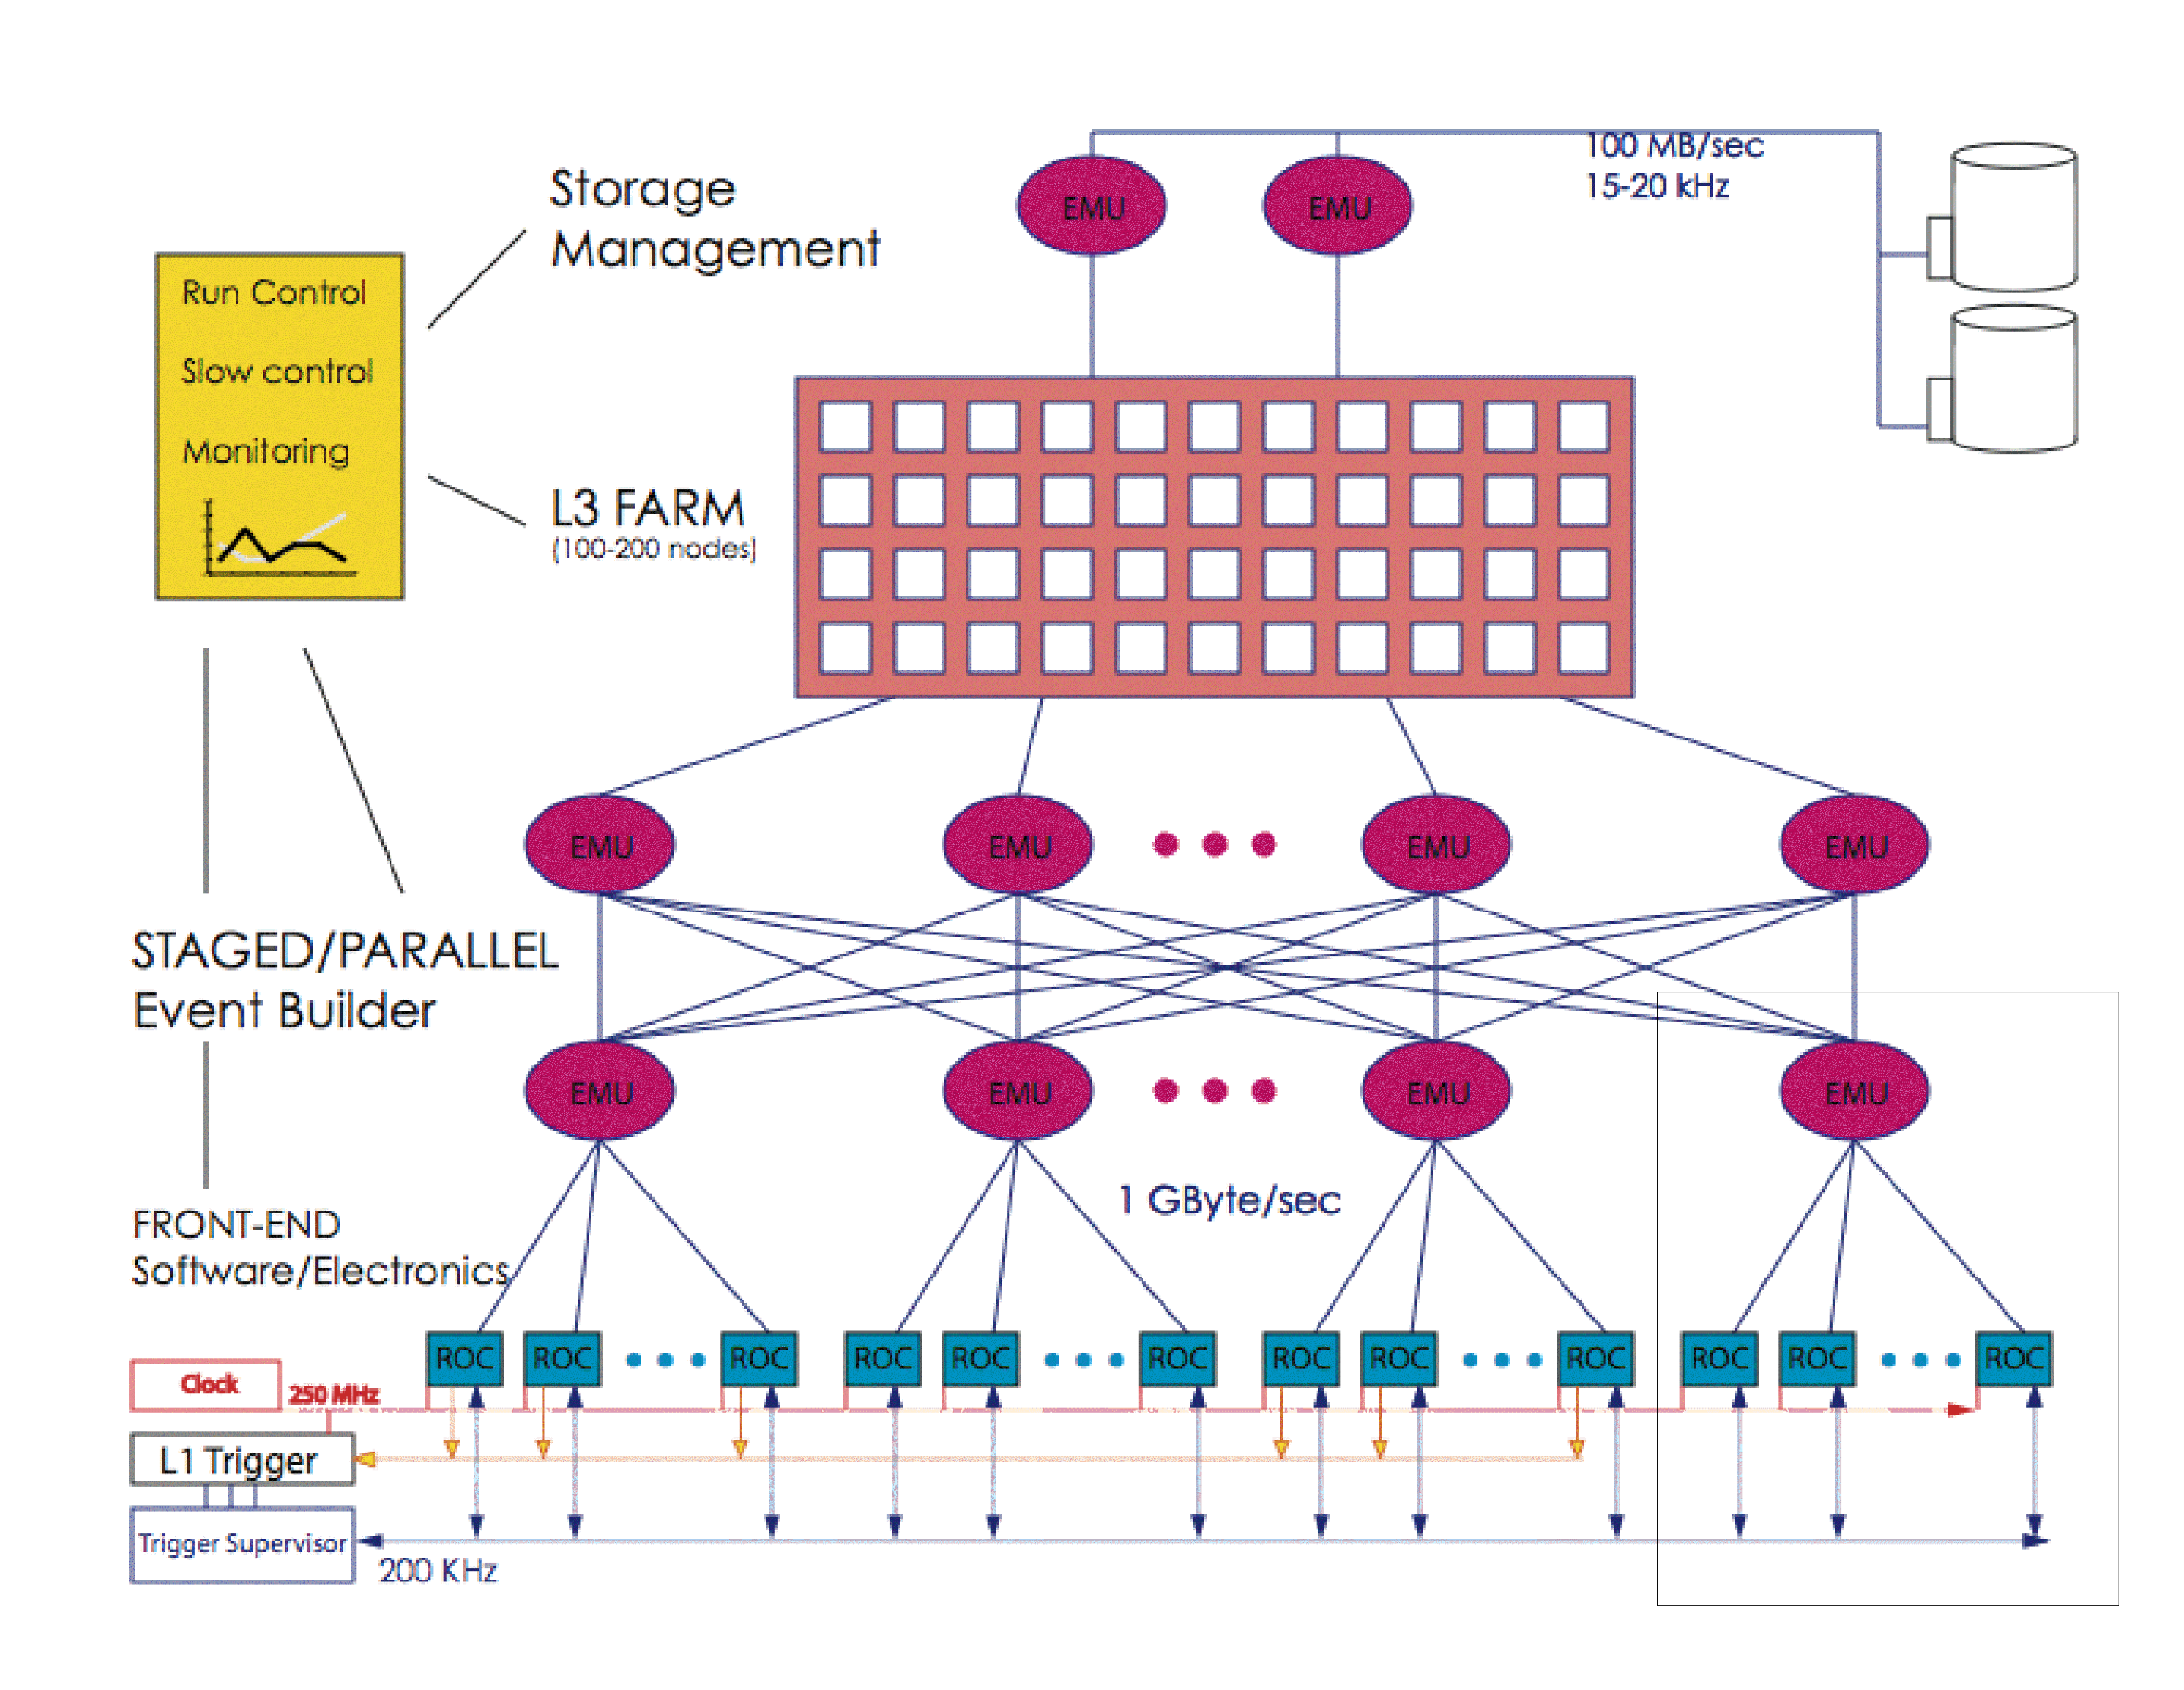
\epsfig{file= DAQ.eps,width=0.95\textwidth}
\end{tabular}
\caption[Lecture 2]{\label{hd10}
Diagram of the Data Acquisition System. The box in the lower right
shows the scale of DAQ systems currently deployed at JLab.}
\end{figure}





%======================== Online Systems =========================

\subsection{Online Systems}


\paragraph{Purpose, Description}


The online effort is the umbrella under which all efforts related to
designing, installing, and
maintaining everything related to controlling and running the
experiment.  These diverse activities will be performed by a small but
dedicated online group mostly residing at JLab.  Below we discuss some
major Online group responsibilities.





CODA, developed by the JLab DAQ group, is essentially a generic
toolkit for producing a high-performance data acquisition systems. It
must be customized and adapted to specific cases.  GlueX will take
innumerable commissioning and data taking runs, and extensive
information about these runs must be recorded along with the data
itself in order to understand how the data should be processed.  This
system has to be developed in its entirety by the Online group.



The task of the Online group is to integrate all components into a
system that allows us to record data and monitor experimental
conditions.  Although the Electronics group will develop the front-end
and trigger hardware, once it is delivered to JLab installation and
commissioning becomes the responsibility of the Online group.



A sophisticated local area network, including fast switches, is
required in the experimental hall to enable movement of 1 GB/sec of
data from the front-end hardware to the event building system.  This
is in addition to the standard network capabilities required by the
experiment control system.  We note that the JLab computer center is
responsible for all networking outside the counting house and
experimental hall, including the special network needed to move 100
MB/sec from local storage in the counting house to permanent storage
in the computer center.



To ensure we will record data of the highest quality, various
monitoring functions are required.  The GlueX DAQ system will provide
a low-rate event stream to an online event monitoring system for
real-time checking and reporting of problems to operators.  
An online event display is indispensible for both commissioning the
detector hardware as it is installed and for debugging hardware
problems as they arise.  It is further useful for analyzing small
numbers of events in real-time.  This system will be developed jointly
by the Online and Analysis groups, as it is quite useful in offline
analysis as well.



The GlueX detector will have many thousands of control points, and 
a flexible, EPICS-compatible controls framework will be chosen.
In addition to the controls system, software systems
must also be monitored and alarms generated when needed.
Examples include failure of the email system or other system
processes, crashing of processor nodes, etc.  We note that the JLab
DAQ group is developing tools to help experimenters create such systems.



Near real-time calibration of event data has proven to be very useful
by many experiments, allowing them to produce physics results quite
soon after data taking.  This system would run in the counting house
on a mini-farm, and would analyze data in real-time.  For running the
experiment at $10^8$ photons/sec the online farm will require
installation of 50-200 farm nodes and associated monitoring equipment,
network design and installation.  The Online group will be responsible
for building and maintaining this farm, and getting data to it as soon
as feasible, while the Software Analysis group will be responsible for
supplying the calibration algorithms themselves.



Finally, we note that some of the tasks above are not specific to
GlueX, and joint development efforts with online groups from other
halls might be very productive.


\paragraph{Current Status, R\&D issues}


Most of the R\&D needed here is being done by other groups, especially
the Electronics, DAQ, and Trigger groups.  For the remainder we will
adapt existing or soon to exist technology (from JLab, CERN, Fermilab,
SLAC, industry, etc.) as needed.  The main effort will go into
customizing the chosen technologies and integrating them into a
coherent and usable online system.  This of course involves quite a
bit of custom code development.




\paragraph{Collaboration Responsibilities}


GlueX will take primary responsibility for the online effort, and we
expect that a large fraction of the work will be done by GlueX staff
and experimenters residing at JLab.  The online software effort is
substantial, involving customization and integration of a wide variety
of outside packages.  The online hardware effort is also substantial,
involving integration of a large number and wide variety of
electronics, computing, and monitoring equipment.  Careful planning
for dedicated manpower is necessary for successful implementation of
the online effort.

Early implementations of the online hardware and software needs to be available two to
three years before the beginning of data taking to allow for detector
and electronics commissioning.





%============== Offline Computing and Software Systems ===============

\subsection{Offline Computing and Software Systems}

The primary goal of GlueX is the systematic identification and
categorization of short-lived meson states, unraveled from the raw,
multi-particle reaction data using the techniques of ``Partial Wave
Analysis" (PWA). Achieving this goal requires simultaneous access to
two large and independent data sets, namely the actual reduced
experimental data and the simulated Monte Carlo data, each sorted for
the particular multi-particle reaction(s) under consideration. It is
quite probable that these data sets will be distributed physically over
multiple locations, and that access will be from other separated
sites, associated with the group who has undertaken that particular
analysis. A schematic diagram of the computing effort is shown in
figure \ref{computing}.



Due to the large volume and complexity of data produced by GlueX
(both experimental and simulated) considerable resources are needed
to manage and analyze the data sets. These can be sorted into two
broad categories: computing infrastructure, and analysis software.


%This not only impacts the structure of the data grid, but also implies
%that new analysis tools need to be developed. This especially includes
%visualization tools, as one searches for the appropriate combination
%of partial waves which best describe the reaction. That is, as one
%fits the parameters associated with a certain set of partial waves,
%some visual inspection mechanism is needed to evaluate how well the
%fit reproduces distributions in angles and invariant mass, for the
%many possible combinations. A universal set of tools is important in
%order to come to a more or less standard set of measures that would be
%applied by the analysis groups.


%======================== Computing Infrastructure =========================

\subsubsection{Computing Infrastructure}


\paragraph{Purpose, Description}


GlueX requires the design and
implementation of a fast backbone network at the lab capable of 
a sustained transfer rate of 100 MB/sec from the counting house to the central
computing facility (CC). In addition, offline storage media will be purchased
and installed in the CC which is capable of handling the approximately 3PB/yr
(1PB/yr raw + 2PB/yr reconstructed+simulated) of data generated by GlueX.
The first
stage data analysis which results in Data Summary Files will be performed
on the large JLab computer farm. The current farm will need to be upgraded
by approximately 450 circa 2008 CPUs in order to satisfy the anticipated
timeline for analyis of GlueX data. Finally, GRID services will be
used for transparent access to the data and resources
at JLab and university computing facilities by GlueX collaborators. This
will require upgrading the JLab internet connection to OC24 or better.



\paragraph{Current Status, R\&D issues}


Much of the above will not be needed for a number of years.  Some of
the items involve extension and/or upgrade of existing facilities,
while others are completely new (e.g. grid services).  JLab is a
member of PPDG (a major grid collaboration) and is actively involved
in grid R\&D.  We note that these all efforts are a continuation of
current computer center activities.



\paragraph{Collaboration Responsibilities}


Development and maintenance of the systems mentioned above will be the
primary responsibility of the JLab Computing Center, although GlueX
collaborators will be involved with the planning effort to
ensure GlueX needs are met.  


We estimate that prototypes of the items above are required
three to five years before the beginning of data taking, and
that production versions should be working one to three years before
data taking (depending on system).  The purchase of
many components (e.g. farm processors, switches, etc.) will be
postponed for as long as possible for economic reasons, but the
infrastructure must be in place early on.

We note that the CEBAF Center extension currently under construction
has dedicted space to house the offline farms and tape storage
facilities needed to support GlueX.



\begin{figure}[h!]\centering
\label{computing}
\begin{tabular}{c}
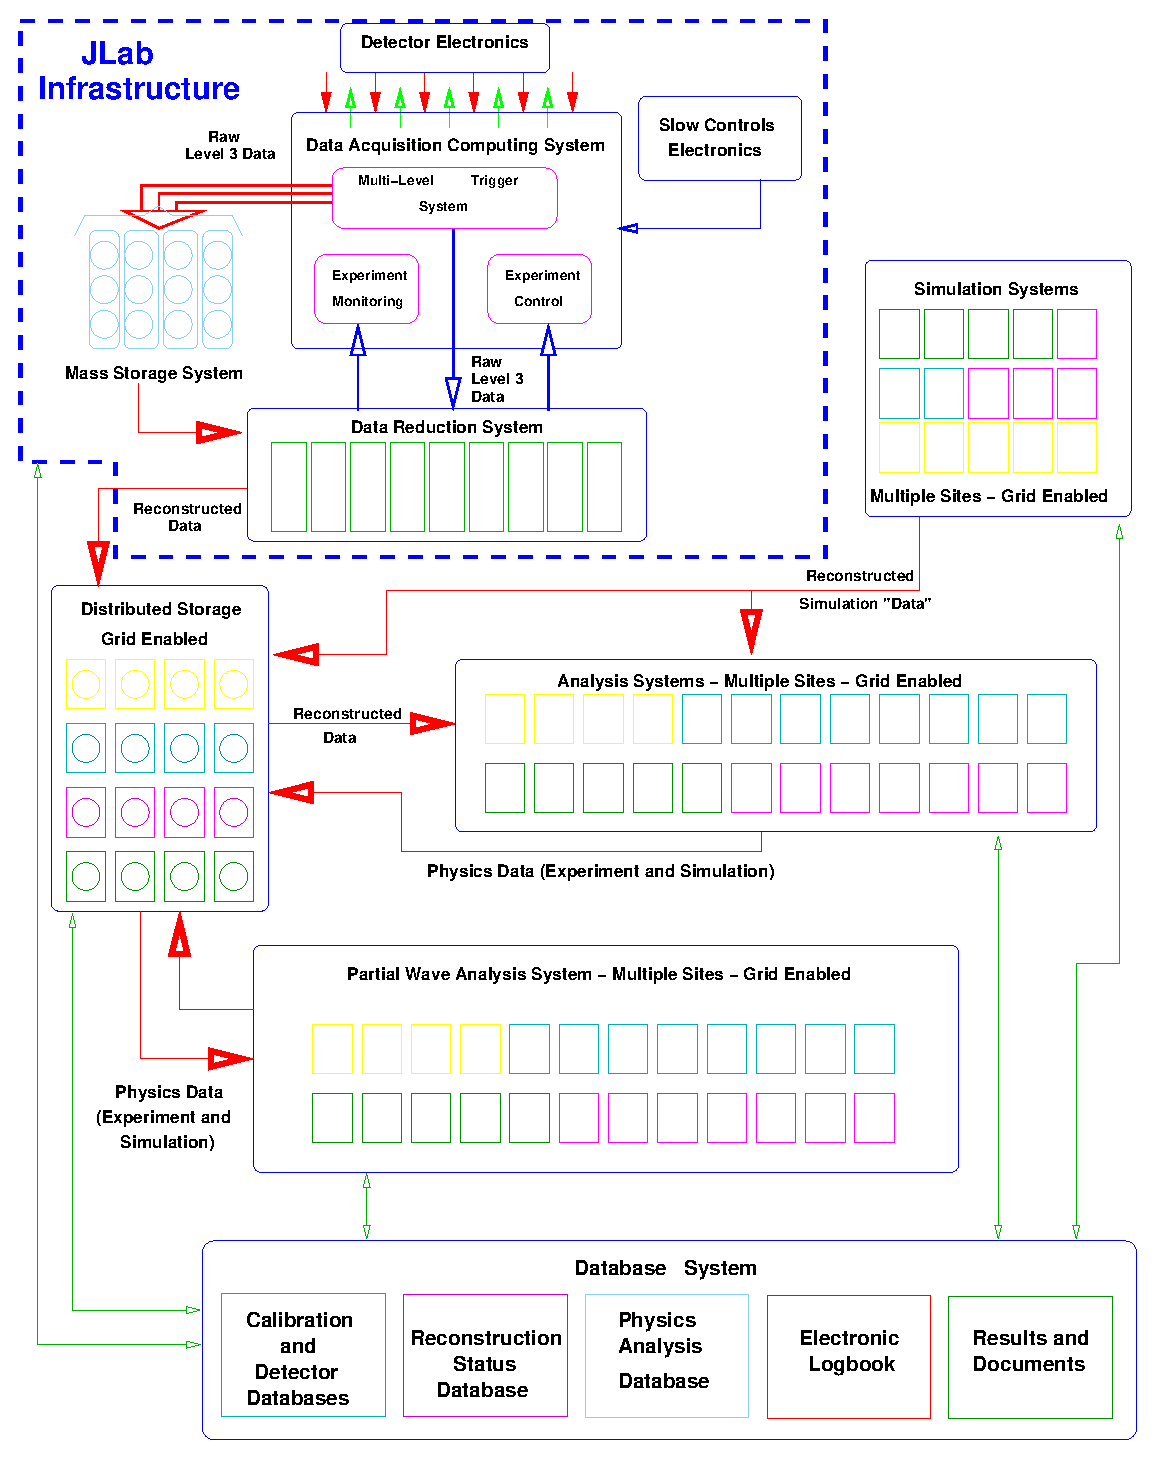
\epsfig{file= ch9_software_systems_small.eps,width=0.95\textwidth}
\end{tabular}
\caption[Lecture 2]{\label{hd10}
The GlueX Computing Environment.}
\end{figure}



%======================== Analysis Software =========================

\subsubsection{Analysis Software}

\paragraph{Purpose, Description}

The analysis software itself can be broken down into three groups:
Simulation, Reconstruction, and Partial Wave Analysis (PWA).


Simulation software will be produced based on
the CERN GEANT package. This will generate data which simulates
the response of each detector to particle interactions. Initially,
the simulated data
will be used to finalize the detector design. It will also be used
to develop the reconstruction software critical to online monitoring
of the data. Finally, a large simulated data set is required
as input to the Partial Wave Analysis.


Reconstruction software will be written for each
detector system. The individual packages will be
combined using a common analysis framework currently under development
within the collaboration. This will involve 
reconstruction of all detector systems including
shower reconstruction in the calorimeters, particle tracking in the 
chambers, and particle identification. A database is required
to hold sets of calibration constants. This will require an 

Application Programming Interface (API) be written for accessing
the values from within the analysis framework. Calibration programs will be
written for each detector system to produce calibration constants and 
submit them to the database.


The level 3 trigger will
implement the reconstruction software to determine
which events to write to tape. This will likely 
need to be a faster (and consequently less accurate) version
of the reconstruction software made to interface with the Data Acquisition
System. The exact algorithm will need to be optimized to filter the data set
as much as possible without introducing any trigger
inefficiencies.


PWA software is currently being
developed for use in analyzing data from existing experiments
(CLAS, E852). PWA will be the final stage of analysis for
the GlueX data. This is a critical and sensitive piece of the
analysis software which will require significant resources
to develop. Input to the PWA
will be in the form of Data Summary Files. These will contain
events which have undergone full reconstruction including
particle identification and kinematic fitting as output
from the reconstruction part of the analysis software.


\paragraph{Current Status, R\&D issues}


GlueX has developed a preliminary simulation suitable for experiment design
and acceptance studies, and has begun work on an offline analysis
framework and on the experiment data model.  GlueX is also a leader in
the world-wide effort to develop new PWA tools and algorithms.  



\paragraph{Collaboration Responsibilities}


Most of the GlueX analysis and simulation algorithms and software
remains to be developed.  This is a very large effort that has already
begun, and it will continue for years after experiment startup.  The
work will be done by the GlueX collaboration, and a large fraction of
GlueX members are expected to contribute.


A full-featured event simulation, analysis framework, and preliminary
reconstruction and analysis software needs to be available two to four
years before the start of data taking. Preliminary calibration software
must be ready about a year before
startup, and the final system must be ready by the time the experiment
begins. Final reconstruction and
analysis software needs to be ready about six months before data
taking for GlueX to succeed in publishing preliminary results within a
year of startup. A prototype level 3 trigger must be available
about one year before startup for testing, but the production level 3
trigger algorithm is not required until later.



\end{document}
